\documentclass[notes,11pt, aspectratio=169]{beamer}
\usetheme{default}
\usepackage[normalem]{ulem}
\renewcommand{\familydefault}{\rmdefault}
\beamertemplatenavigationsymbolsempty
\definecolor{oxfordblue}{RGB}{0,32,68}
\setbeamertemplate{footline}[frame number]{}
\setbeamercolor{title}{parent=oxfordblue}
\setbeamercolor{title}{fg=oxfordblue}
\setbeamercolor{subtitle}{parent=oxfordblue}
\setbeamercolor{date}{parent=oxfordblue}
\setbeamercolor{institute}{parent=oxfordblue}
\setbeamercolor{section title}{parent=oxfordblue}
\setbeamercolor{subsection title}{parent=oxfordblue}
\setbeamercolor{frametitle}{parent=oxfordblue}
\setbeamercolor{background canvas}{parent=oxfordblue}
\setbeamercolor{structure}{fg=oxfordblue}
\setbeamercolor{normal text}{fg=black!97}
\setbeamercolor{footnote}{fg=black!97}
\setbeamercolor{page number in head/foot}{fg=oxfordblue}
\setbeamerfont{caption}{size=10}
\usepackage{mathtools}
\usepackage{amsmath}
\usepackage{bbm}
\usepackage{dirtytalk}
\usepackage{booktabs}
\usepackage{tabularx}
\usepackage{comment}
\usepackage{csquotes}
\usepackage{float}
\usepackage{caption}
\usepackage{subcaption}
\usepackage{graphicx}
%\usepackage[authoryear]{natbib}
%\addbibresource{references.bib}
\usepackage[
backend=biber,
style=authoryear-comp,
]{biblatex}
%\title{A bibLaTeX example}
\addbibresource{references.bib} 

%\setlength{\parindent}{0in}
%\usepackage{calc}
%\usepackage[export]{adjustbox}


\title{
Credit Cards and Retail Firms: \newline 
Historical Evidence from the U.S.}
\author{Joseph Hall}
%\insertdate{<year}{<month>}{day}
\date{\today}
%\newdate{date}{06}{09}{2012}
%\date{\displaydate{date}}
\institute{Georgia Institute of Technology}

\titlegraphic{
\includegraphics[scale = 3]{Static/qr_website.png}}
\makeatletter
\setbeamertemplate{title page}{%
  \vbox{}
  \begingroup
    \centering
    \begin{beamercolorbox}[sep=8pt,center]{title}
      \usebeamerfont{title}\inserttitle\par%
      \ifx\insertsubtitle\@empty%
      \else%
        \vskip1.5em%
        {\usebeamerfont{subtitle}\usebeamercolor[fg]{subtitle}\insertsubtitle\par}%
      \fi%
    \end{beamercolorbox}%
    \vskip1em\par
    \begin{beamercolorbox}[sep=8pt,center]{author}
      \usebeamerfont{author}\insertauthor
    \end{beamercolorbox}
    \begin{beamercolorbox}[sep=8pt,center]{institute}
      \usebeamerfont{institute}\insertinstitute
    \end{beamercolorbox}
    \begin{beamercolorbox}[sep=8pt,center]{date}
      \usebeamerfont{date}\insertdate
    \end{beamercolorbox}%\vskip0.5em
  \endgroup
}
\makeatother\usepackage[utf8]{inputenc}

\begin{document}
\bgroup
\makeatletter
\setbeamertemplate{footline}
{
  \leavevmode%
  \hbox{%
}%
  \vskip0pt%
}
\makeatother
\begin{frame}
\titlepage
%\includegraphics[scale = 0.01]{Figures/qr.png}

\end{frame}
\egroup

\setcounter{framenumber}{0}


\begin{frame}{}

\textbf{Research Question}: Have credit card networks benefited retail firms?

\begin{center}
\large
    \textbf{Roadmap} 
\end{center}

\begin{enumerate}
    \item \textbf{Document Trends}: Banks have replaced retail firms as suppliers of short-term consumer credit in the U.S. since 1958
    \item \textbf{Causal Identification}: Natural experiment shows that this increases firms' profits and relieves them of risk
    \item \textbf{Mechanisms and Model}: Structural model with firm-level data to answer: 
    \begin{itemize}
        \item What determines firms' choice to accept cards?
        \item How large is the net cost reduction?
        \item How much do credit payment options affect consumer choice over retailers?
    \end{itemize}
\end{enumerate} \vfill 
\textbf{Main Finding}: Firms accept bank cards to reduce costs by about 3\%, which benefits both firms and consumers 

\end{frame}


\begin{frame}{Historical Context}

\small 

    ``Most Americans had a dozen or more different forms of credit... an account at the neighborhood pharmacy, the neighborhood grocery store, and a half-dozen other local stores''
    \newline 
    ``It was the smaller merchants who first came around... The man almost kissed my feet... His accounts receivable were dragging him under''
    \newline 
     ``I looked at the size of his accounts: \$4.58. \$12.82.\footnote{Inflation since 1958 $\approx$ 10x} He was sending out monthly bills. Then the customers paid him maybe three or four months later''
     \newline 
    ``The bank would guarantee him payment--within days instead of months--and would take over the role of collecting from the customers... [while] taking a 6 percent cut.'' 

   \flushright -Bank of America salesman, 1958, on enrolling merchants (\cite{nocera_piece_2013})
\flushleft 
\vfill \pause 
``A dozen or more'' in 1958 is down to 3.2 avg cards today, down from 4 in 1990 (SCF) despite a threefold increase in spending share on cards 
    
\end{frame}

%I kinda don't like this slide -- can I make it my own rather than one giant quote? 


\begin{frame}{Why Might Firms Not Benefit?}

Two Reasons: 
\begin{itemize}
    \item Bank, especially if monopoly, may be able to charge more than cost savings (\cite{rochet_platform_2003}, \cite{edelman_price_2015}, \cite{wang_regulating_2023})
    \item Interoperable credit cards issued by banks may make firms better substitutes and force them to lower prices 
\end{itemize}

\vfill \pause 

Same as asking ``are merchant fees too high for the real service merchants receive?'' 

\vfill \pause 

A (small) change in profits is equal to: 

\begin{equation}\label{eq:decomposition3}
    \underbrace{\frac{d\mathrm{\pi}}{PQ}}_\mathrm{Change\,in\,Profit\,Rate} = \underbrace{- \left(\sigma-1\right) \mu  \frac{dC}{C}}_\mathrm{Change\,due\,to\,Cost} + \underbrace{d\mu}_\mathrm{Change\,in\,Markup}
\end{equation}

Where $P \equiv \left(1 + \mu \right)C $ and $\sigma \equiv -\frac{\partial Q}{ \partial P} \frac{P}{Q}$
    
\end{frame}


\begin{frame}{Roadmap}

\textbf{Section 1: Aggregate Trends}
\begin{itemize}
    \item Bank credit rose and displaced store credit 
    \item Stores spend less on credit-related labor 
\end{itemize}

\textbf{Section 2: Identification of Real Effects}
\begin{itemize}
    \item An unexpected Supreme Court ruling in 1978 affected bank card supply differently across states 
    \item Bank card usage rose, store credit fell, profitability increased, and firms already on bank card network lost sales
\end{itemize}

\textbf{Section 3: Mechanisms, Structural Model}
\begin{itemize}
    \item Discrete-choice model of consumer choice over retailers
    \item Model allows credit to change \textbf{costs} and \textbf{markups} as free parameters 
    \item Simulated Method of Moments to fit model to results from part (2) 
\end{itemize}
    
\end{frame}



\begin{frame}[label = literature]{Related Literature}

\small \textbf{Credit Expansions} \tiny \cite{beck_finance_2008}, \cite{beck_big_2010}, \cite{chatterji_entrepreneurial_2012}, \cite{cuesta_price_2021}, \cite{kroszner_regulation_2014}, \cite{jayaratne_entry_1998}, \cite{kroszner_what_1999}, \cite{chong_effects_1991}, \cite{schularick_credit_2012}, \cite{mian_what_2014}, \cite{mian_how_2020}, \cite{julia_fonseca_how_nodate}, \cite{herkenhoff_impact_2021}
\small 
\begin{itemize}
    \item Formal credit may crowd out informal 
    \item Case of tech-driven credit boom (this tech: verification at distance and scale)
\end{itemize}
 
\small \textbf{Credit Bundling and Trade Credit} \tiny \cite{banner_competition_1958}, \cite{brennan_vendor_1988}, \cite{benetton_credit_2022},  \cite{low_auto_2020},  \cite{murfin_who_2019}
\small 
\begin{itemize}
    \item Non-durable products, atomistic consumers (unlike B2B)
    \item Correlation between demand shocks and default suggests undiversified retailers should be particularly \emph{poor} holders of own customers' default risk 
\end{itemize}
 
\small \textbf{IO of Payments} \tiny \cite{rochet_platform_2003}, \cite{edelman_price_2015}, \cite{wang_regulating_2023}, \cite{brunnermeier_mobile_2023}, \cite{agarwal_real_2020}, \cite{huynh_equilibrium_2022}, \cite{arango_consumer_2015}, \cite{evans_paying_2004}
\small 
\begin{itemize}
    \item Quantitative evidence of aggregate impact when technology can change costs 
\end{itemize}
    
\end{frame}


\begin{frame}{Preview of Main Findings}

\begin{enumerate}
    \item Store cards (non-interoperable, with firms bearing default risk) were 75\% of credit card spending in 1970, but 10\% in 2020.
    \item More than half of bank credit growth caused by the end of usury (maximum interest rate) regulation in 1978 substituted for less retail lending. 
    \item In net, this increased firm profits and net entry of retail firms 
    \item A model estimates that this reduced retail industry's net cost by about 3\%, dominating firms' lost markups from interoperability 
    \begin{itemize}
        \item The net effect of bank cards is positive for firm profits and consumer surplus
        \item This is only true because banks are much more efficient than firms at credit supply, and the estimated importance of interoperability is small
    \end{itemize}
\end{enumerate}

        
\end{frame}


\begin{frame}{Data Sources}

\begin{itemize}
    \item \textbf{Consumer Credit Use}: Survey of Consumer Finance 
    \vfill 
    \item \textbf{Firm Credit Supply and Profits}: Census QFR (industry-level), Compustat (firm-level) 
    \vfill 
    \item \textbf{Sales and Survival by Location}: Dun and Bradstreet (establishment-level)
    \vfill 
    \item \textbf{Net Entry}: US Census County Business Patterns (establishment-level)
    \vfill 
    \item \textbf{Usury Regulation}: ``Cost of Personal Borrowing in the United States'' (state-level)
    \vfill \pause 
    \item \textbf{Bank Card Acceptance}: Yellow Pages (New establishment-level data)
\end{itemize}
    
\end{frame}


\begin{frame}{New Data on Bank Card Acceptance}
\begin{center}
    
\begin{columns}[T] % align columns
\begin{column}{.3\textwidth}
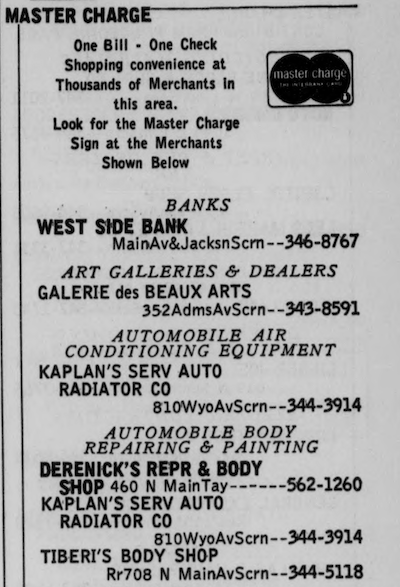
\includegraphics[scale = 0.3]{Static/yellowpages_mc.png}    
\end{column}
\hfill 
\begin{column}{.2\textwidth}
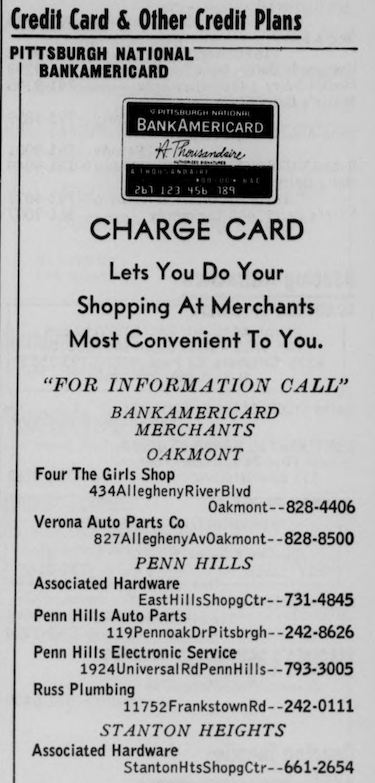
\includegraphics[scale = 0.22]{Static/yellowpages_visa.png}    
\end{column}
\end{columns}
\vfill 
Source: U.S. Telephone Directory (``USTD'') Collection, Library of Congress
\end{center}
\end{frame}

\begin{frame}{Data Collection}

\begin{itemize}
    \item \textbf{Step 1}: Identify 1,155 business directories since 1950 comprising 3,130 region-years from universe of Library of Congress Online directories  
    \item \textbf{Step 2}: Identify 378 instances of explicit bank card acceptance listings comprising 25,519 firm-years
    \item \textbf{Step 3}: Link to Dun and Bradstreet establishment-level panel using phone numbers, addresses, and business names (2,956 unique firms; 81\% of listings which overlap with D\&B coverage)
\end{itemize}
\hyperlink{coverage_time}{\beamergotobutton{Coverage in Time}} \hyperlink{coverage_geographic}{\beamergotobutton{Coverage over Counties}}

%Add many click-throughs here 
\end{frame}


\section{Aggregate Trends}
    \begin{frame}[noframenumbering, plain]
        \vfill
      \centering
      \begin{beamercolorbox}[sep=8pt,center,shadow=true,rounded=true]{title}
        \usebeamerfont{title}\insertsectionhead\par%
        \color{oxfordblue}\noindent\rule{10cm}{1pt} \\
      \end{beamercolorbox}
      \vfill
\end{frame}


\begin{frame}{Bank Cards Displaced Store Credit}

\begin{center}
\begin{columns}[T] % align columns
\begin{column}{.4\textwidth}
    From the household perspective 
    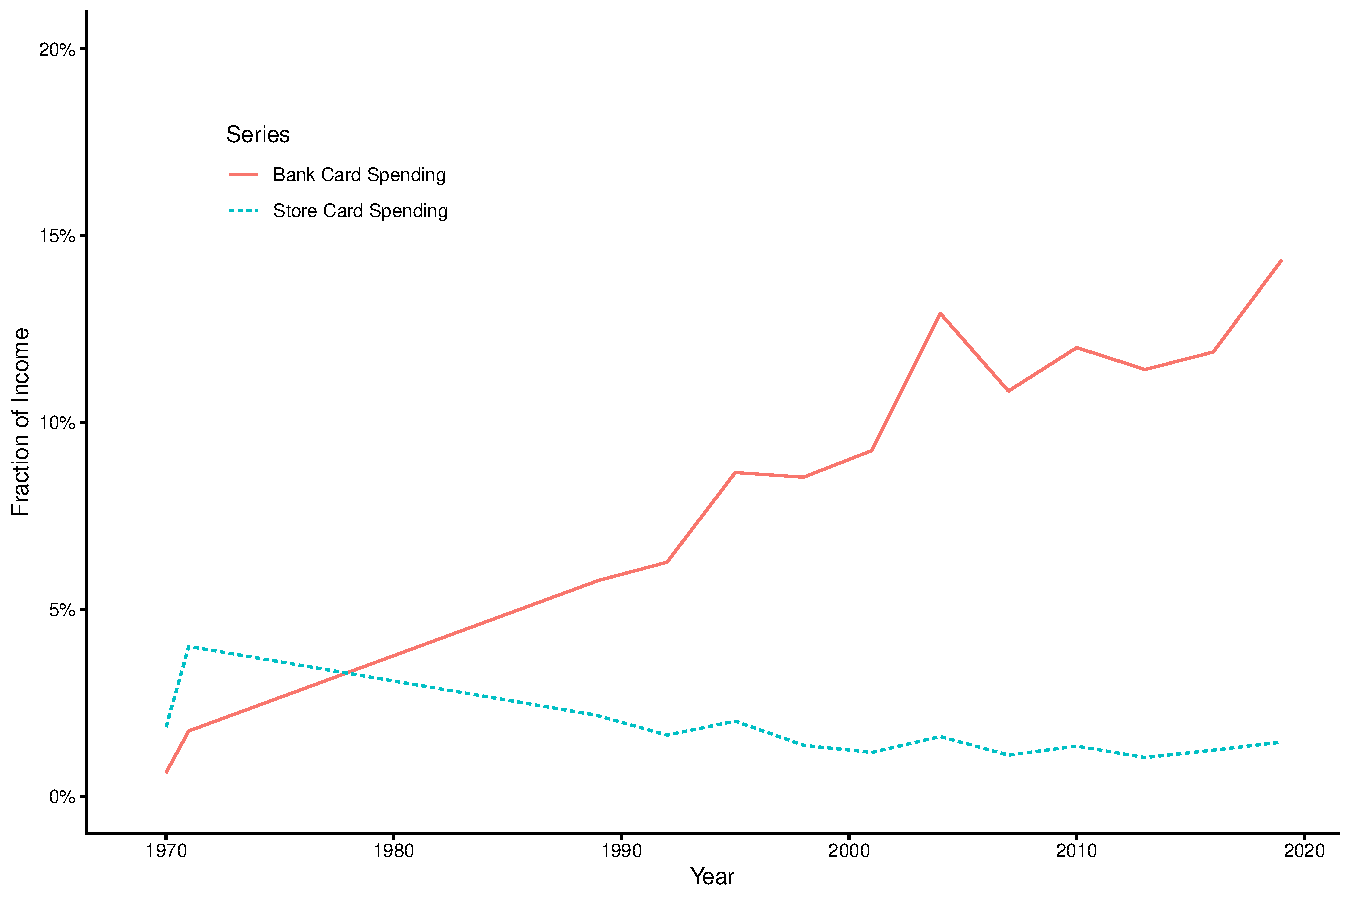
\includegraphics[scale = 0.4]{../Output/Figures/spending_levels.pdf}    
    Source: SCF
\end{column}
\hfill  \pause 
\begin{column}{.4\textwidth}
    And from the firm perspective 
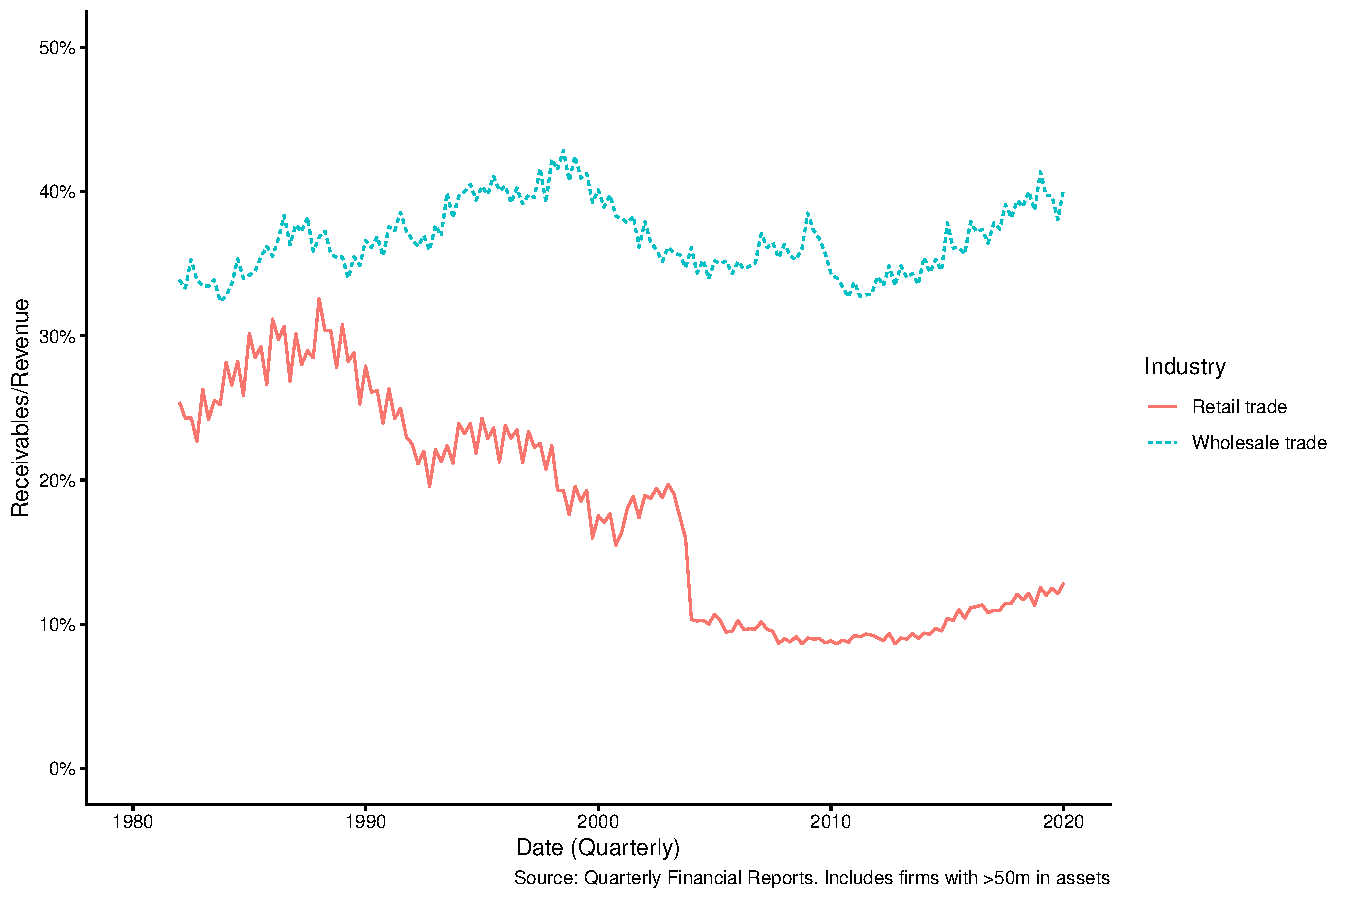
\includegraphics[scale = 0.3]{../Output/Figures/receivables.pdf}    
    Source: US Census
\end{column}
\end{columns}
\end{center}
\end{frame}


\begin{frame}[label = wage_bill]{Labor Cost Reductions}

Retail firms once spent 4\% of their wage bill on ``bookkeepers and bill collectors'' 

\begin{center}
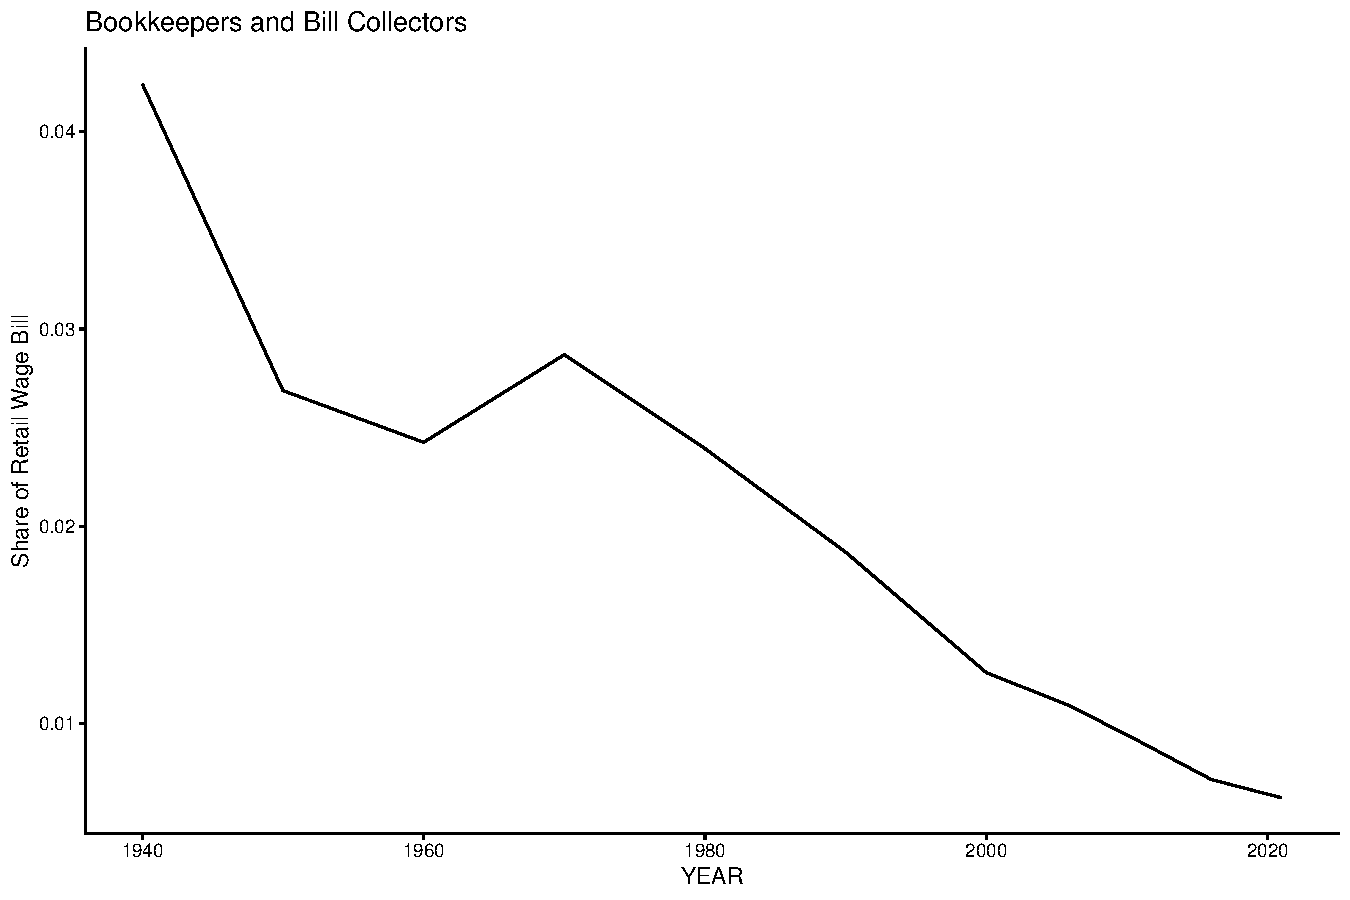
\includegraphics[scale = 0.3]{../Output/Figures/backoffice_retail.pdf}
\end{center}
\tiny \begin{center}
    Source: US Census  
\end{center} 
\normalsize
\begin{itemize}
    \item 78\% drop since 1970, compared to 63\% drop in wholesale sector 
\end{itemize}

%\hyperlink{risk_sharing}{\beamergotobutton{Additional Evidence}}

\end{frame}


\section{Identification: Abolition of Usury Limits}
    \begin{frame}[noframenumbering, plain]
        \vfill
      \centering
      \begin{beamercolorbox}[sep=8pt,center,shadow=true,rounded=true]{title}
        \usebeamerfont{title}\insertsectionhead\par%
        \color{oxfordblue}\noindent\rule{10cm}{1pt} \\
      \end{beamercolorbox}
      \vfill
\end{frame}

\begin{frame}{The Equilibrium Effect of Bank Cards}

\textbf{Goal}: estimate the effect of bank credit card usage on firm outcomes

This requires variation in bank credit card supply that is: 

\begin{itemize}
    \item Is not confounded by other forms of credit (e.g. mortgages, commercial loans)
    \item Is not confounded by credit demand 
    \item Varies across markets
    \item Is unanticipated 
\end{itemize}
\vfill  
The 1978 \emph{Marquette} decision by the U.S. Supreme Court creates such an ideal source of variation

\end{frame}


\begin{frame}{1978 \emph{Marquette} decision}
\begin{itemize}
 \item In 1978, supreme court ruled banks can lend across state lines at their home state's usury rate (maximum legal interest rate)
 \vfill 
 \item Banks located in deregulated states expanded lending to consumers in regulated states
 \vfill 
 \item Large banks such as Citibank and Bank of America migrated HQ's to no-limit states (South Dakota and Delaware, respectively) in 1981-1982
 \vfill
 \item Revolving credit (cards) regulated separately from installment loans -- no effect on, e.g., mortgages and industrial loans 
 \vfill 
 \item Suggests a \textbf{single-treatment-time} Difference-in-Difference design with standard parallel trends assumption 
\end{itemize}  
\end{frame}

\begin{frame}{Support for Parallel Trends: Usury rates varied idiosyncratically in 1977}

\begin{centering}
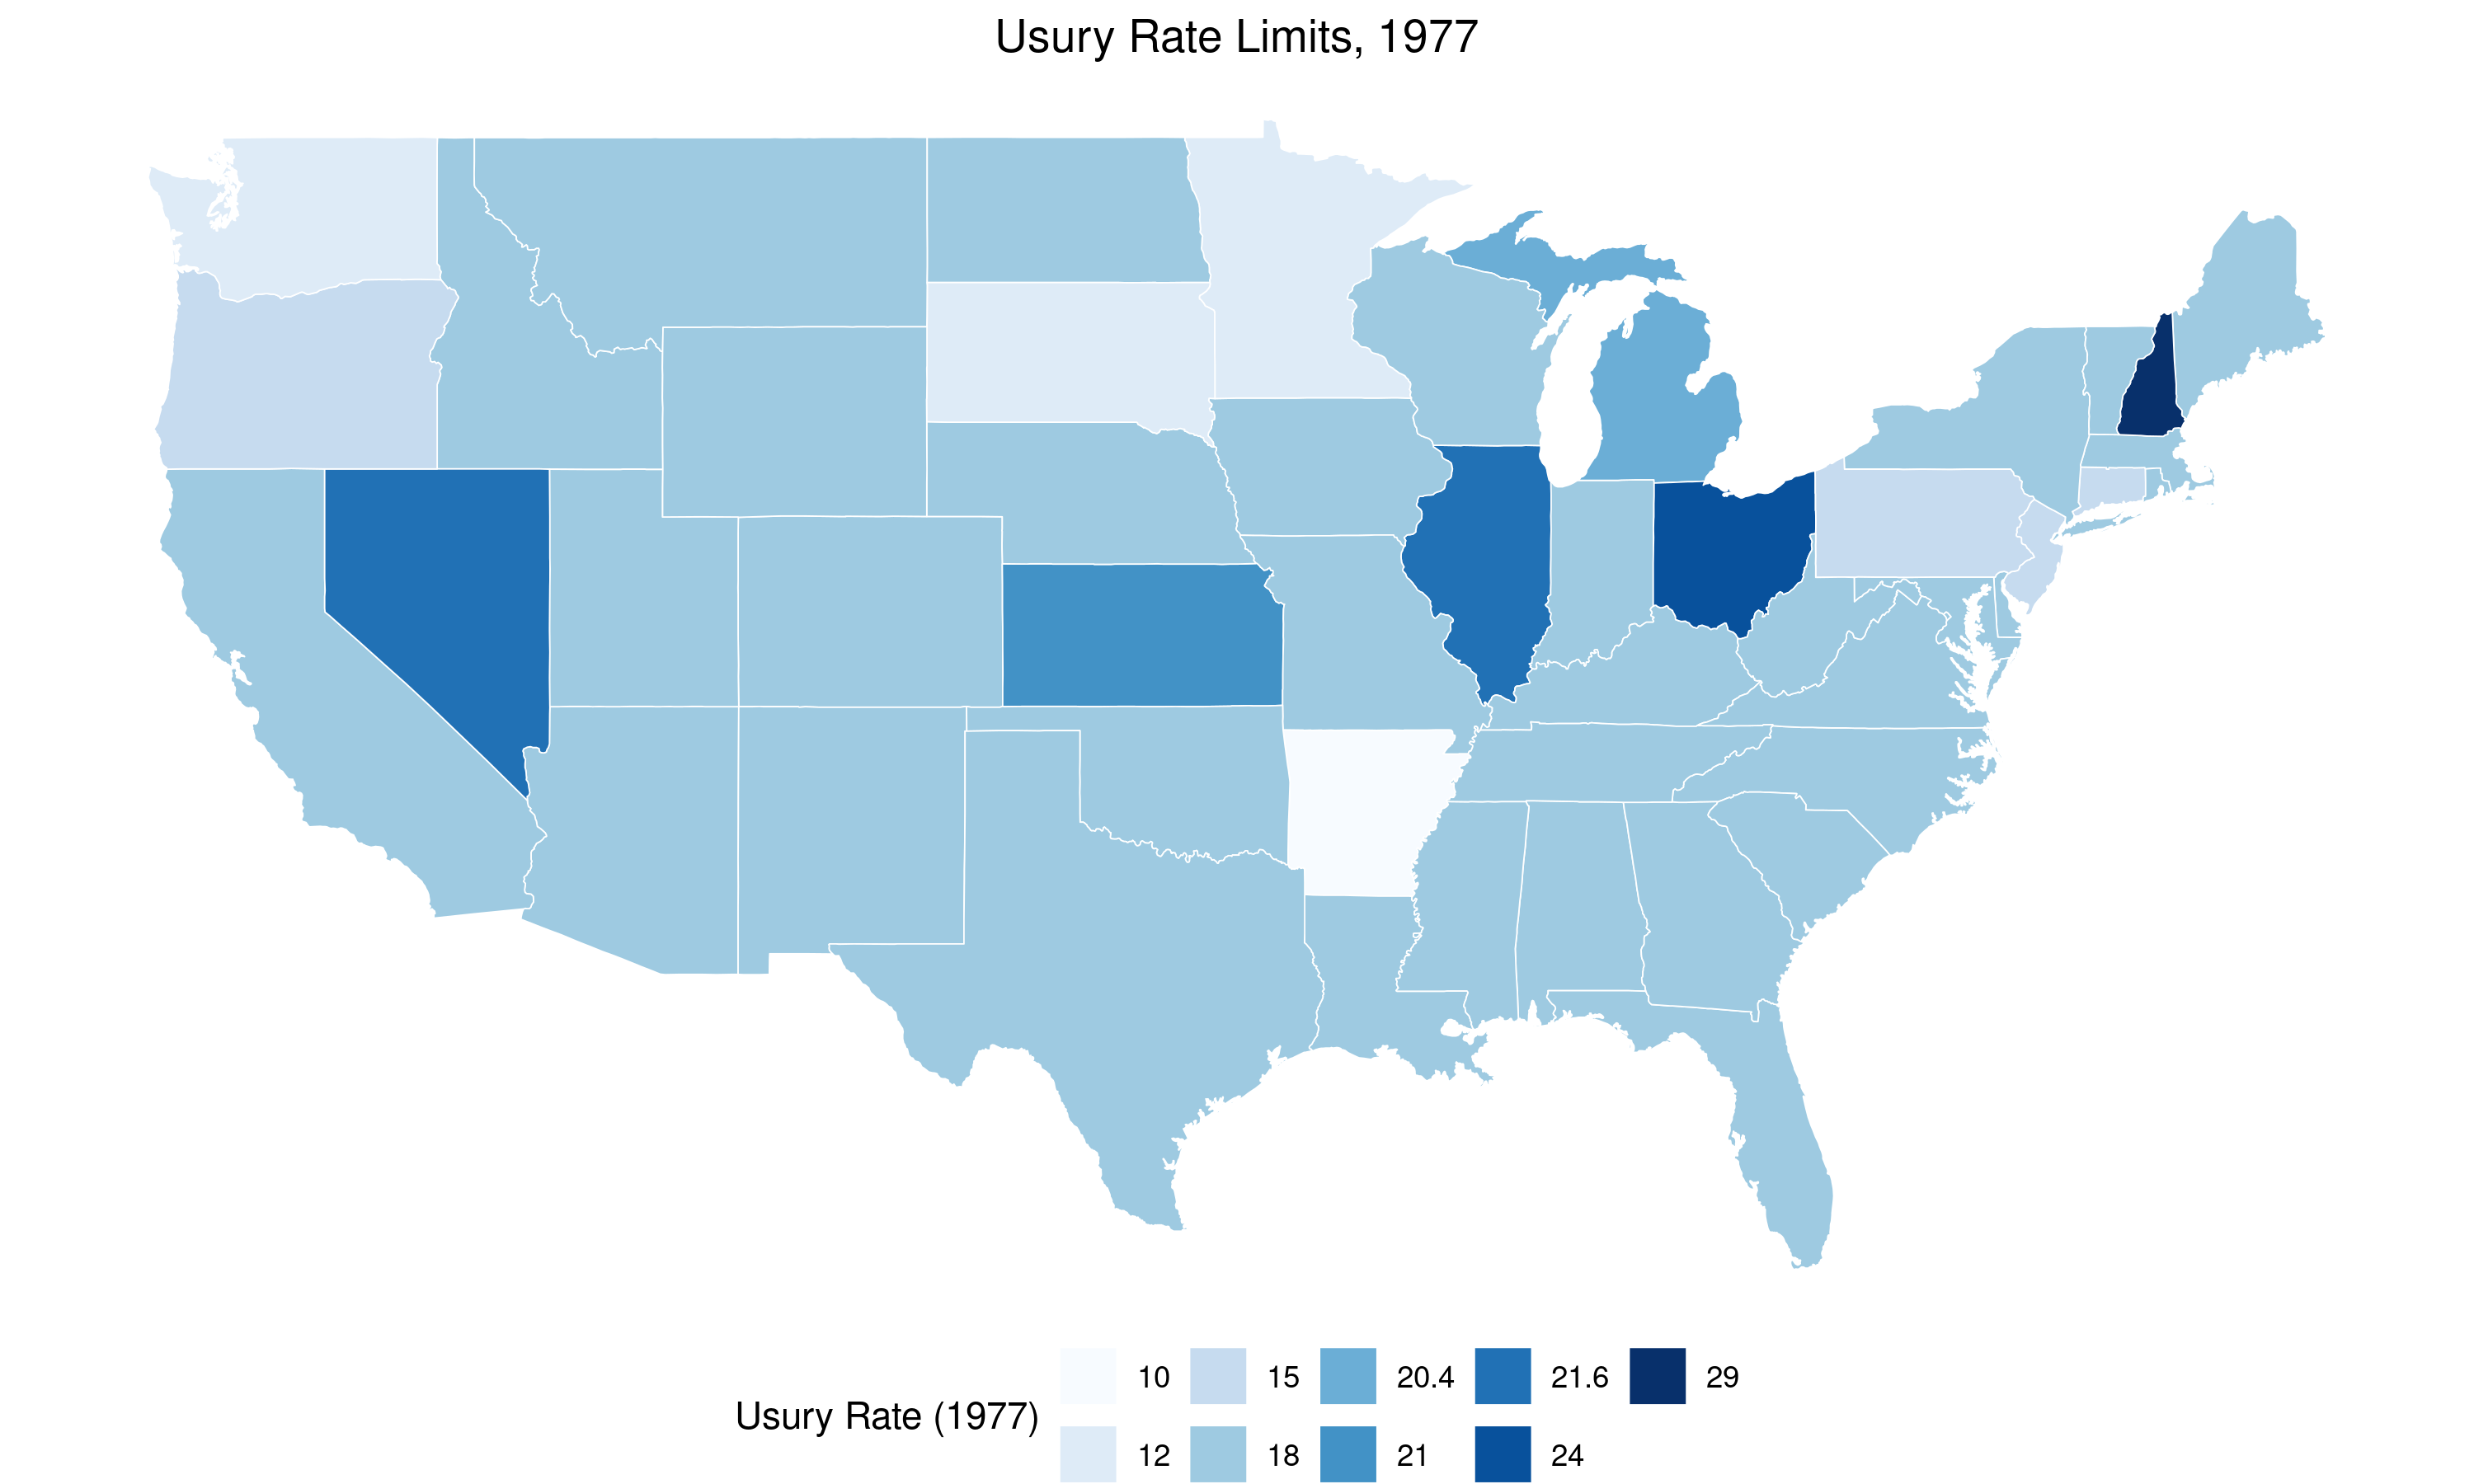
\includegraphics[scale = .55]{../Output/Figures/rate_77.png} \\
\end{centering}
Source: \emph{Cost of Personal Borrowing in the United States}, 1977
\pause 
\begin{itemize}
    \item Correlates -0.04 with \cite{mian_how_2020} index of 1970-1990 deregulation and macro credit growth 
\end{itemize}
\end{frame}


\begin{frame}[label = bunching]{Relevance: usury regulation was tightly binding}

\begin{columns}[T]
\begin{column}{.5\textwidth}
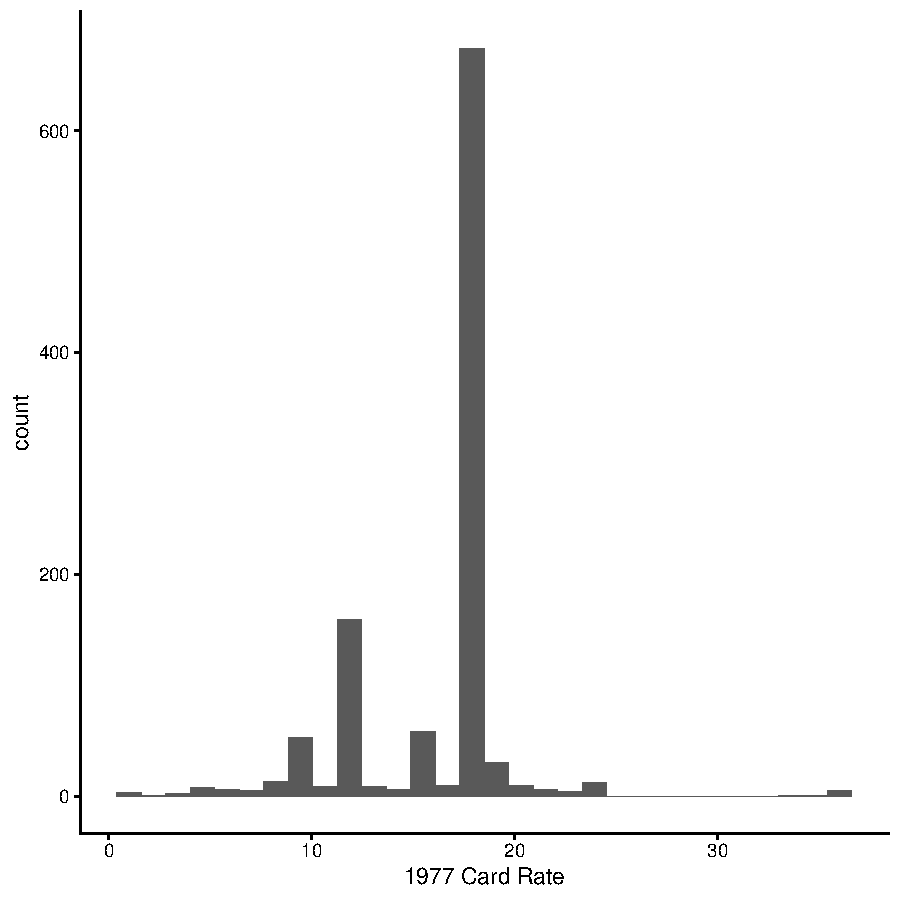
\includegraphics[scale = 0.45]{../Output/Figures/bunching}
\end{column}
\begin{column}{.5\textwidth}
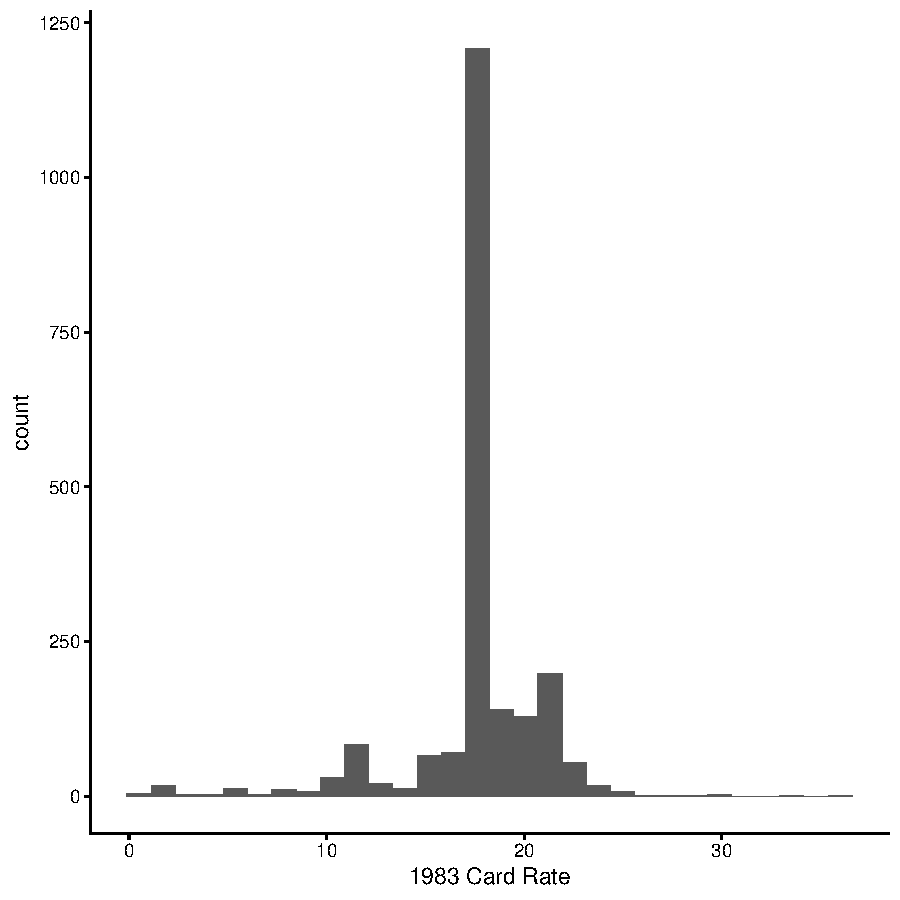
\includegraphics[scale = 0.45]{../Output/Figures/bunching_83}
\end{column}
\end{columns}

%\hyperlink{binding_limit}{\beamergotobutton{Back}}

\end{frame}

\begin{frame}{Relevance: usury regulation was tightly binding}
    
    \begin{centering}
    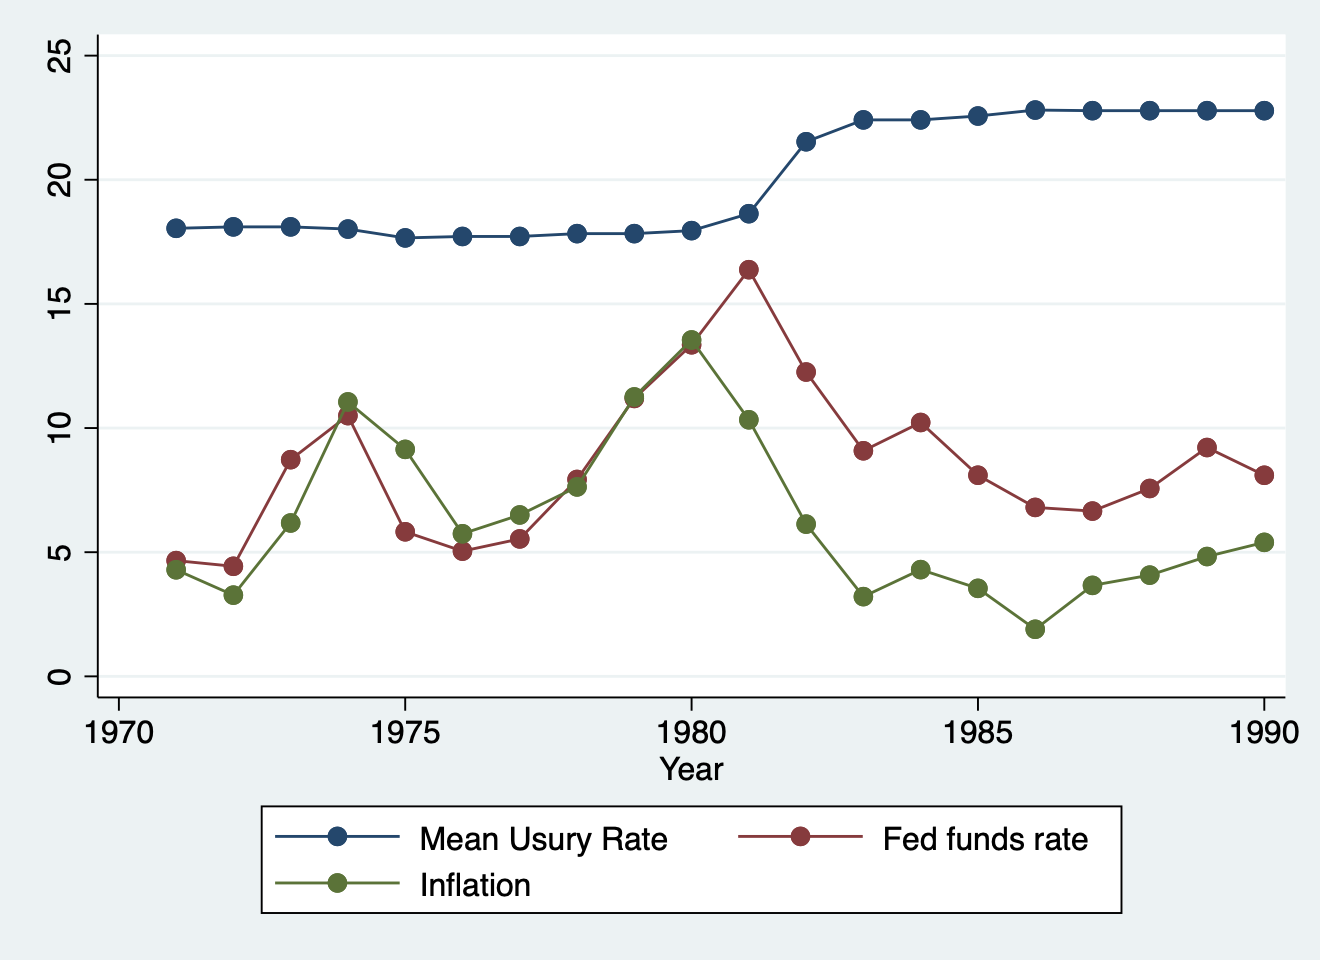
\includegraphics[scale = .36]{Static/usury_rate.png} \\
    \end{centering}
    \begin{itemize}
        \item Usury lending rate was barely above inflation and fed funds rate (lower limit of bank marginal cost)
    \end{itemize}
\end{frame}

\begin{frame}[label = rise]{}
    \centering
    \textbf{Growth in Aggregate Bank Card Lending}
  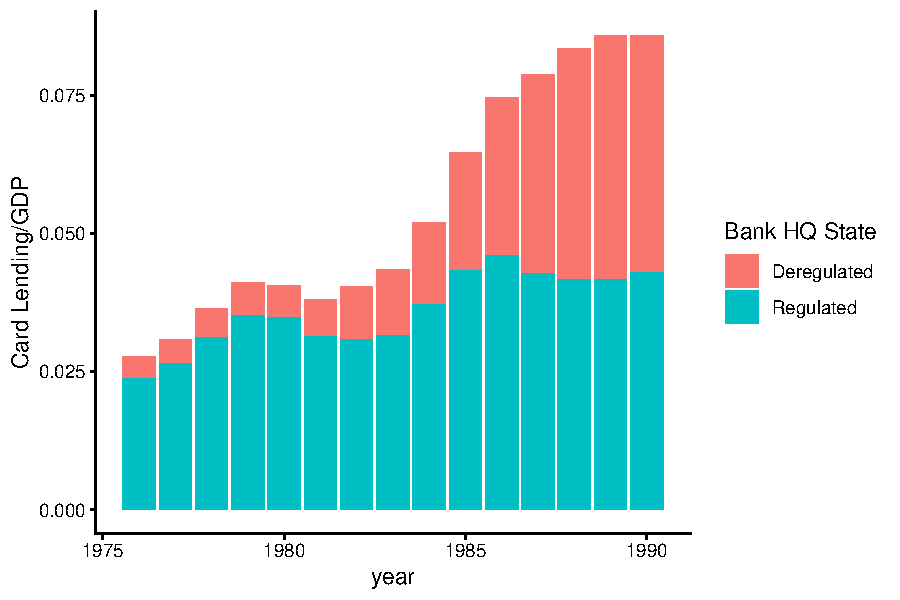
\includegraphics[scale=.65]{../Output/Figures/card_growth_stacked.pdf}
    \begin{itemize}
        \item 13 states removed usury limits by 1982
    \end{itemize}
\end{frame}

\begin{frame}{Main estimating equation}

I use a dynamic differences-in-differences design: 

$$Y_{it} = \alpha_i + \alpha_t + \beta_{t\ne 1977} T_i + \varepsilon_{it}$$

\begin{itemize}
    \item \textbf{Comparison}: markets where customers suddenly had access to more bank cards vs. where bank cards had already been widely available 
    \pause 
    \item $Y_{it}$ are various outcomes of interest 
    \item $i$ are states/counties/firms (data permitting), $t$ are years
    \item $T_i$ is 1 if the state had a usury limit below 18\% in 1978 
    \begin{itemize}
        \item \cite{zinman_impact_2003} finds a 5.5 pp increase in bank card holding in affected states from 1977 to 1983 using this treatment definition %(quasi-``first-stage'' for my reduced form)
        \item 9 ``treated'' states representing 37 million Americans (16\% of nation)
    \end{itemize}
    \item Single treatment time means traditional two-way fixed effects DiD is not biased by time-varying treatment effects
    \item Std. errors clustered by state (\cite{abadie_when_2017})
\end{itemize}    
\end{frame}



\begin{frame}{Receivables of Multi-Establishment Firm}

Receivables are tracked at the firm-level, but many firms sell in many states 

\vfill 
I calculate the firm-level treatment of firm $i$ which has sales $SLS_e$ establishments $e$ in states $s(e)$ as a weighted average:

$$T_i = \sum_e \frac{T_{s(e)} \times SLS_{e}}{\sum_e SLS_e}$$
    
\end{frame}

\begin{comment}
    \begin{frame}{Preview of Causal Results}

Three key facts causal facts the model's estimates of \textbf{cost reduction} and \textbf{interoperability}: 

\begin{enumerate}
    \item Change in Receivables 
    \begin{itemize}
        \item How large was the mass of firms who switched?
        \item Data available at the firm level, aggregated across sales locations
    \end{itemize}
    \item Change in Profits 
    \begin{itemize}
        \item Key to disciplining the size of the cost reduction 
        \item Data at firm level
    \end{itemize}
    \item Relative change in sales for firms already on bank card network
    \begin{itemize}
        \item Key to separating interoperability from cost reduction 
        \item Intuition: Firms already on network face intensified competition 
        \item Data at local establishment level 
    \end{itemize}
\end{enumerate}
    
\end{frame}
\end{comment}


\begin{frame}{Retailers Reduced Lending}

    \begin{center}
          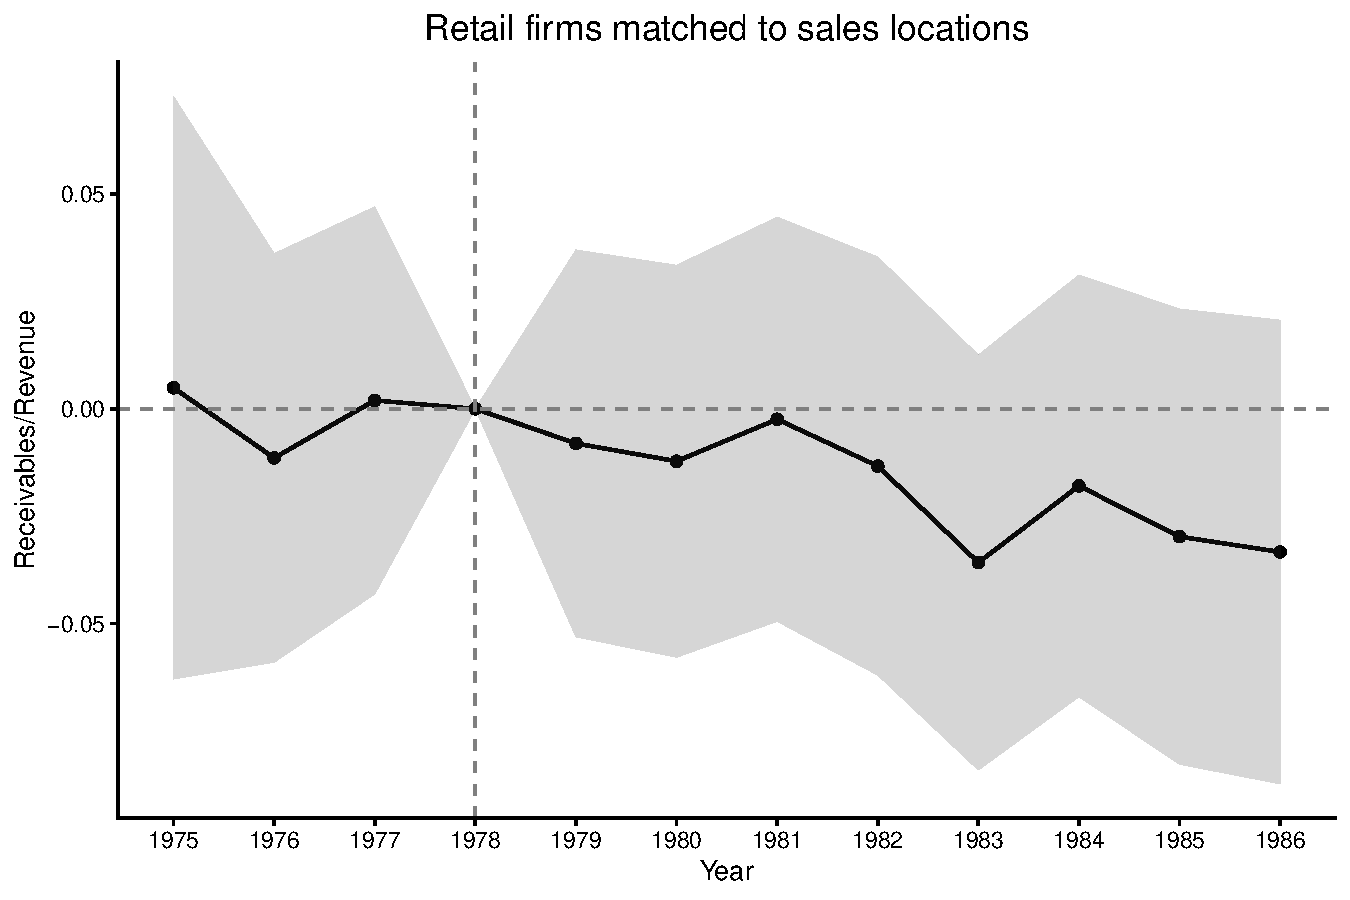
\includegraphics[width=.7\textwidth]{../Output/Figures/receivables_revenue.pdf}
    \end{center}
  Data: All 185 retail firms covered by Compustat in 1978

\end{frame}


\begin{frame}{Accounting Profits Increased}

\small 

\begingroup
\centering
\begin{tabular}{lc}
   \tabularnewline \midrule \midrule
   Dependent Variable:    & Net Income / Revenue\\  
   Model:                 & (1)\\  
   \midrule
   \emph{Variables}\\
   Treated $\times$ Post  & 0.0091$^{*}$\\   
                          & (0.0054)\\   
   \midrule
   \emph{Fixed-effects}\\
   Year FE                & Yes\\  
   Firm FE                & Yes\\  
   \midrule
   \emph{Fit statistics}\\
   Observations           & 2,000\\  
   R$^2$                  & 0.21338\\  
   Within R$^2$           & 0.00058\\  
   \midrule \midrule
   \multicolumn{2}{l}{\emph{Clustered (Firm FE) standard-errors in parentheses}}\\
   \multicolumn{2}{l}{\emph{Signif. Codes: ***: 0.01, **: 0.05, *: 0.1}}\\
\end{tabular}
\par\endgroup




\end{frame}


\begin{frame}{Triple Differences by Use of Cards for Transactions}

Regression on accounting net income suffers several deficiencies: 

\begin{itemize}
    \item ``Consumer'' credit cards may allow entrepreneurs to start businesses, or increase demand (\cite{mian_how_2020})
    \item GAAP Net Income may not equal economic profits 
    \item Few firms with public accounting data in 1977
\end{itemize}

\vfill \pause 

I address these with a triple-difference specification: 

$$Y_{it} = \alpha_i + \alpha_t + \beta_{1,t\ne 1977} T_i + \beta_{2,t\ne 1977} T_i Clothing\_Industry_i+ \varepsilon_{it}$$

Using establishment counts from Census CBP as $Y_{it}$

\vfill \pause 

Under what assumption is $\beta_2$ a better estimate?
\begin{itemize}
    \item Credit cards are equally useful to entrepreneurs in all industries
    \item Credit cards are more useful for payments in the clothing industry (empirically true)
    \item Net entry is a good proxy for economic profits 
\end{itemize}    
\end{frame}


\begin{frame}{Bank Card Acceptance Across Industries in 1970}
\begin{columns}[T] 
\begin{column}{.4\textwidth}
\begin{table}
\centering
\caption{Credit Card Acceptance by Industry, Scranton 1971}
\centering
\begin{tabular}[t]{llr}
\toprule
industry & acceptance & n\\
\midrule
Food & 6\% & 150\\
Auto & 13\% & 110\\
Clothing & 100\% & 95\\
Hardware & 10\% & 30\\
Misc. & 0\% & 177\\
\addlinespace
Furnishing & 0\% & 63\\
Restaurants & 0\% & 200\\
Department Stores & 0\% & 48\\
\bottomrule
\end{tabular}
\end{table}

\vfill 
\end{column}
\hfill 
\begin{column}{.4\textwidth}
\begin{tabular}[t]{lll}
\toprule
Card use & Store cards & Bank cards\\
\midrule
Clothing & 84\% & 54\%\\
Appliances & 15\% & 9\%\\
Misc. & 15\% & 38\%\\
Household goods & 14\% & 5\%\\
Recreation items & 8\% & 5\%\\
\addlinespace
Hardware & 5\% & 5\%\\
Furniture & 4\% & 10\%\\
Travel & 0\% & 27\%\\
\bottomrule
\end{tabular}

\vfill 
\end{column}
\end{columns}    

Cross-industry heterogeneity in card usage from new firm side data (left) aligns with consumer-side SCF (right)

\end{frame}


\begin{frame}{Net Entry of Clothing Retail Firms}
\begin{columns}[T] % align columns
\begin{column}{.35\textwidth}

\makebox[\linewidth][c]{
    \resizebox{\linewidth}{!}{
      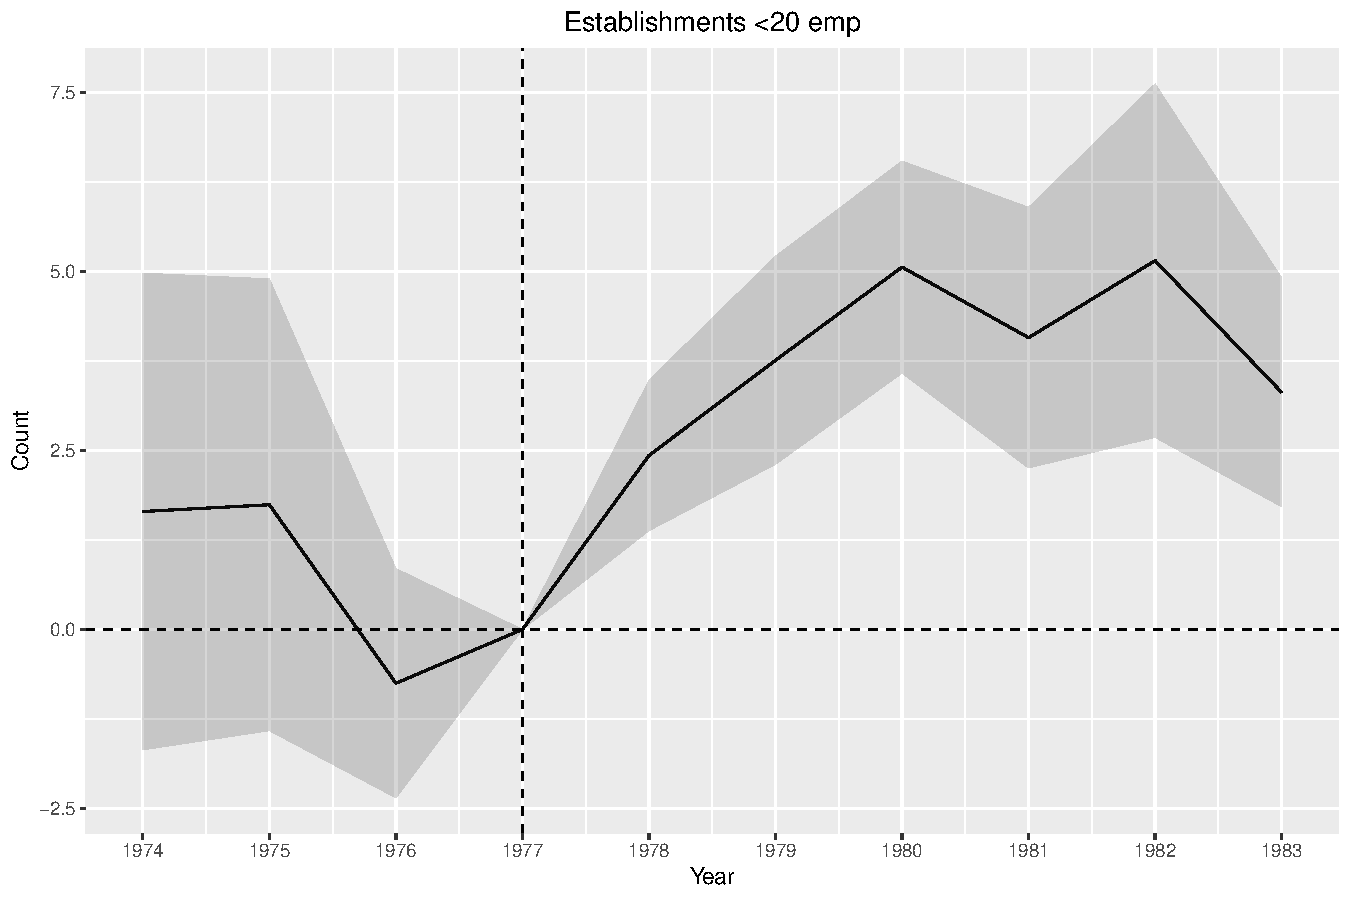
\includegraphics{../Output/Figures/n1_19.pdf}
    }
  }
\end{column}
\hfill%
\begin{column}{.35\textwidth}
  \makebox[\linewidth][c]{
    \resizebox{\linewidth}{!}{
      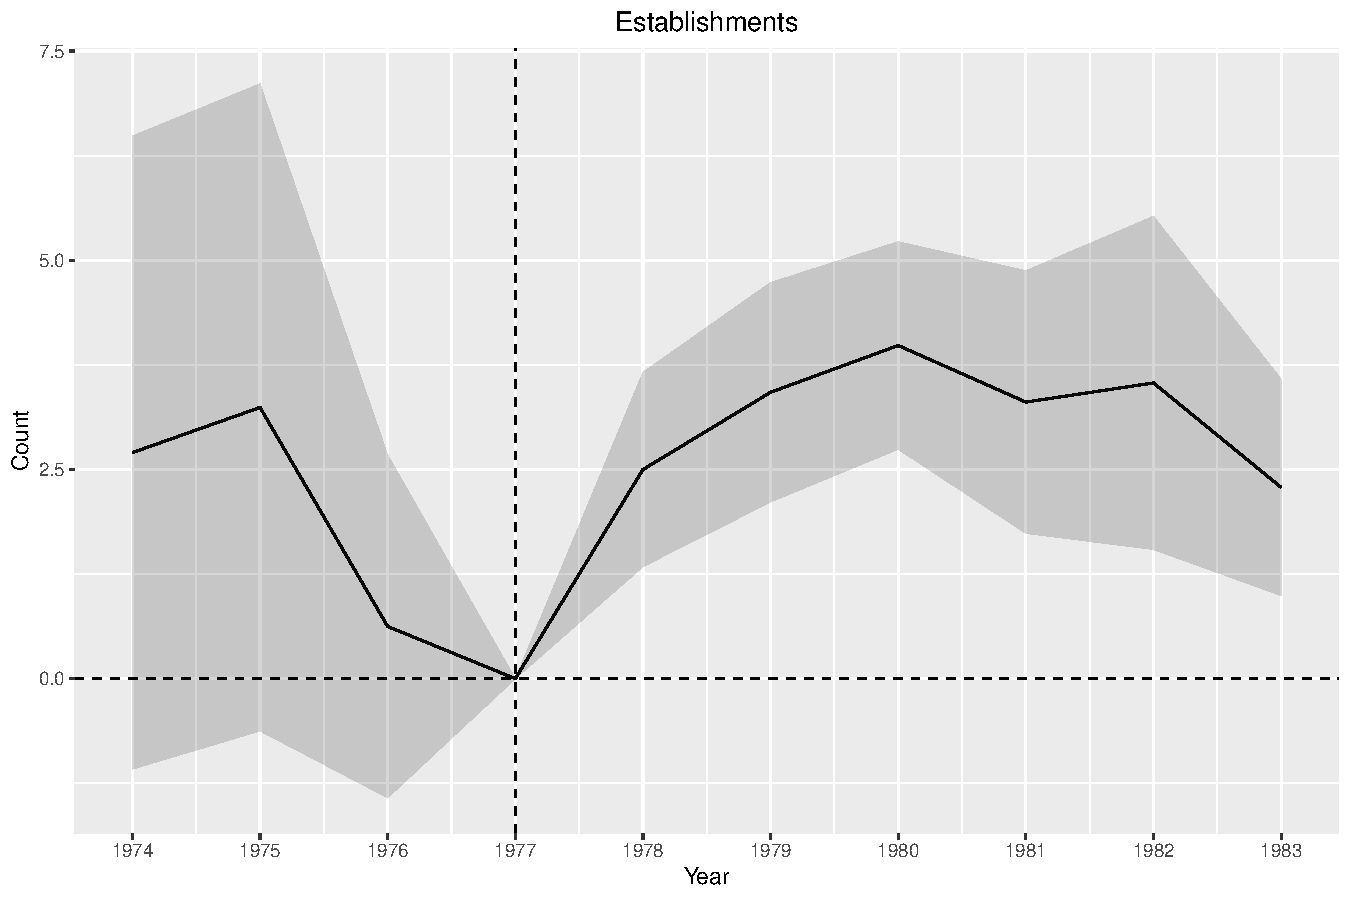
\includegraphics{../Output/Figures/est.pdf}
    }
  }
\end{column}%
\hfill%
\begin{column}{.35\textwidth}
  \makebox[\linewidth][c]{
    \resizebox{\linewidth}{!}{
      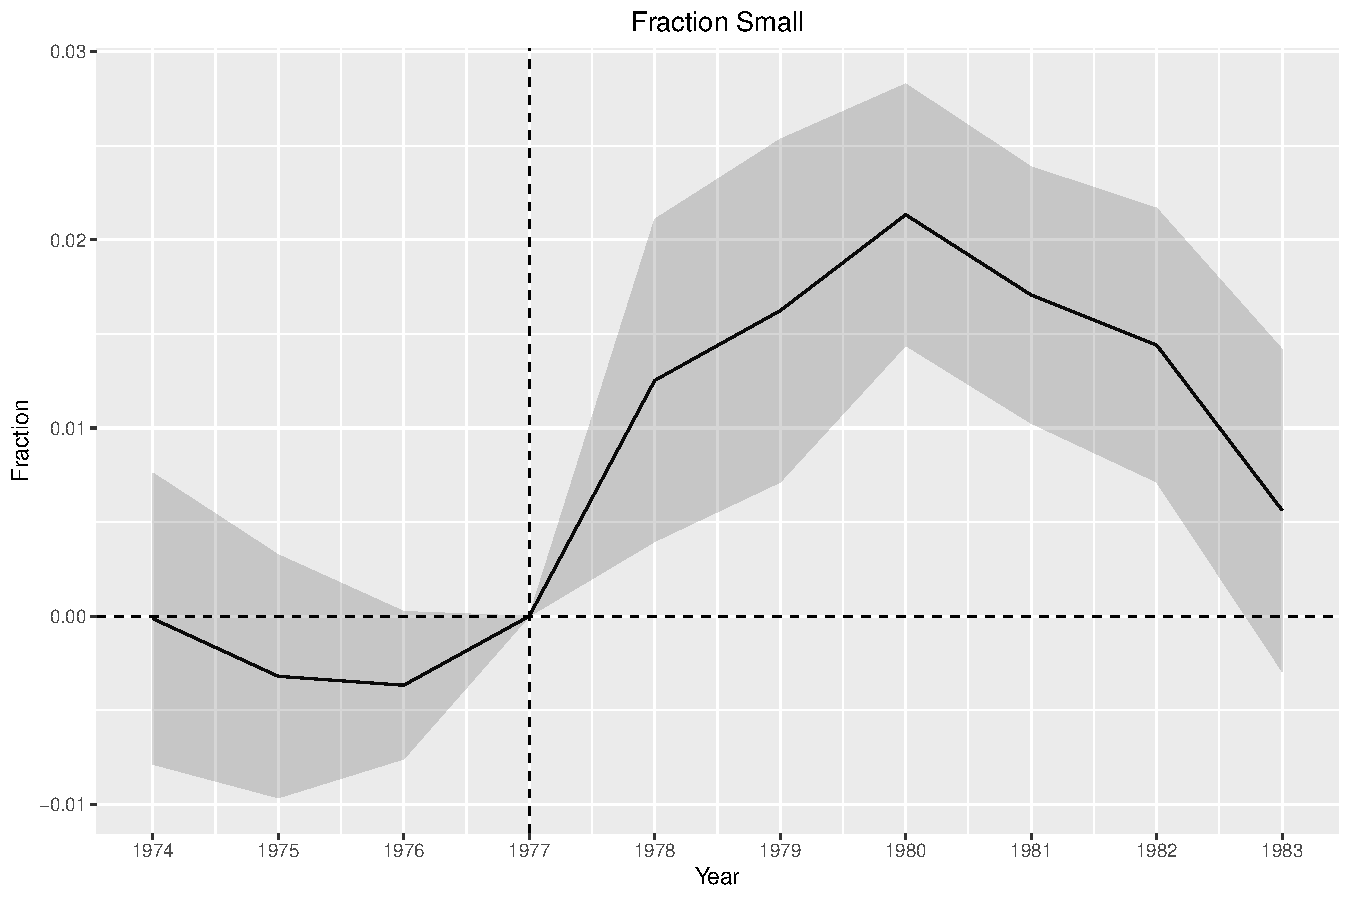
\includegraphics{../Output/Figures/frac_small.pdf}
    }
  }
\end{column}%
\end{columns}
Data Source: County Business Patterns at County-Sic Code-Year level. 
\begin{itemize}
    \item Increase due to small firms -- consistent with economies of scale in the provision of store credit 
\end{itemize}

\end{frame}


\begin{frame}{Effect on Sales and Survival} 

\begin{itemize}
    \item Which firms are early adopters of bank credit cards? 
    \item How do existing card-accepting businesses respond to greater use of the network?
    \item Card networks advertise increased sales for merchants %Click through here
    \item Analyze D\&B Establishment-level sales panel 
    \begin{itemize}
        \item Each market is a city x 4-digit-SIC
        \item Regress growth rates from 1977-1983 on treatment x pre-acceptance 
        \item Survival times also a proxy for profitability 
    \end{itemize}
\end{itemize}
    
\end{frame}

%NEED AN EXPLANATION SLIDE HERE

\begin{frame}{Which Firms Adopt Cards?}

\small 
\begingroup
\centering
\begin{tabular}{lcc}
   \tabularnewline \midrule \midrule
   Dependent Variable: & \multicolumn{2}{c}{Card acceptance}\\
   Model:                     & (1)            & (2)\\  
   \midrule
   \emph{Variables}\\
   log(Sales)                 & 0.7112$^{***}$ & 0.7243$^{***}$\\   
                              & (0.1500)       & (0.1505)\\   
   Single-establishment       & 0.6874$^{***}$ & 0.7132$^{***}$\\   
                              & (0.2410)       & (0.2308)\\   
   Firm age                   &                & -0.0075\\   
                              &                & (0.0071)\\   
   \midrule
   \emph{Fixed-effects}\\
   Industry $\times$ City FE  & Yes            & Yes\\  
   \midrule
   \emph{Fit statistics}\\
   Observations               & 1,940          & 1,940\\  
   Squared Correlation        & 0.23179        & 0.23384\\  
   Pseudo R$^2$               & 0.24409        & 0.24501\\  
   BIC                        & 1,522.3        & 1,528.6\\  
   \midrule \midrule
   \multicolumn{3}{l}{\emph{Clustered (industry) standard-errors in parentheses}}\\
   \multicolumn{3}{l}{\emph{Signif. Codes: ***: 0.01, **: 0.05, *: 0.1}}\\
\end{tabular}
\par\endgroup


\begin{itemize}
    \item Geographically-concentrated, high-volume, long-established businesses 
\end{itemize}

\end{frame}

\begin{frame}{How do Card-Accepting Businesses Respond?}

\small 
\begingroup
\centering
\begin{tabular}{lcccc}
   \tabularnewline \midrule \midrule
   Dependent Variables: & Sales growth & Survival (years) & \multicolumn{2}{c}{Sales growth}\\
   Model:                       & (1)            & (2)           & (3)            & (4)\\  
   \midrule
   \emph{Variables}\\
   Accepts bank card                   & 0.0188$^{***}$ & -0.0194       & 0.0007         & 0.0193$^{***}$\\   
                                & (0.0002)       & (0.1885)      & (0.0028)       & (0.0013)\\   
   Log sales, 1977                  & -0.0037        & 0.1777$^{**}$ & -0.0038        & -0.0039\\   
                                & (0.0057)       & (0.0346)      & (0.0056)       & (0.0057)\\   
   Accepts card $\times$ Treated  & -0.0231$^{**}$ & 0.8225$^{**}$ &                & -0.0237$^{***}$\\   
                                & (0.0044)       & (0.1604)      &                & (0.0036)\\   
   Treated                      &                &               & -0.0074$^{**}$ & -0.0042$^{**}$\\   
                                &                &               & (0.0013)       & (0.0010)\\   
   \midrule
   \emph{Fixed-effects}\\
   State                        & Yes            & Yes           &                & \\  
   Industry (SIC)                         & Yes            & Yes           & Yes            & Yes\\  
   \midrule
   \emph{Fit statistics}\\
   Observations                 & 525            & 525           & 525            & 525\\  
   R$^2$                        & 0.32740        & 0.18762       & 0.32613        & 0.32697\\  
   Within R$^2$                 & 0.00328        & 0.01944       & 0.00326        & 0.00451\\  
   \midrule \midrule
   \multicolumn{5}{l}{\emph{Clustered (State) standard-errors in parentheses}}\\
   \multicolumn{5}{l}{\emph{Signif. Codes: ***: 0.01, **: 0.05, *: 0.1}}\\
\end{tabular}
\par\endgroup

\normal 
\begin{itemize}
    \item Better survival despite \emph{decrease} in dollar revenue consistent with cost channel 
\end{itemize}
    
\end{frame}

\begin{frame}{Firm Resiliency to Risk}

1975 and 1983 major spikes in unemployment before and after \emph{Marquette}: 

\begin{figure}[htp!]
    %\caption{Unemployment Rate and Recessions since 1948}\label{fig:recessions}
    \begin{center}
    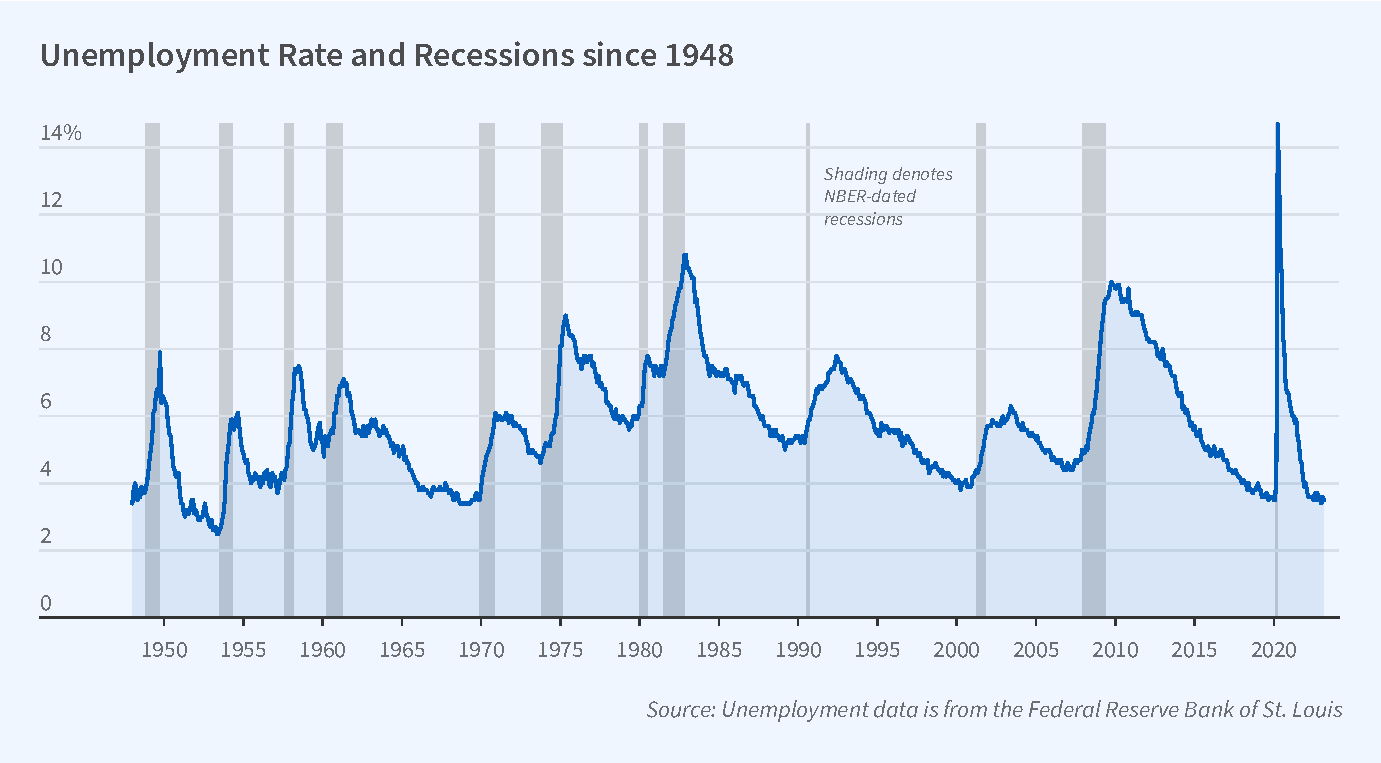
\includegraphics[width = .84\textwidth]{Static/unemployment-rate-and-recessions-since-1948.pdf}
    \end{center}
    %\newline \noindent \small \uline{Source:} NBER
\end{figure}
    
\end{frame}

%Need another slide here explaining the subsequent regression 

\begin{frame}{Firm Survival During Recessions}
    \begin{table}[!ht]{}
    \tiny 

\label{tab:dif-dif-recession}

\begingroup
\centering
\begin{tabular}{lcccc}
   \tabularnewline \midrule \midrule
   Dependent Variable: & \multicolumn{4}{c}{Exit rate}\\
   Model:                                              & (1)             & (2)             & (3)             & (4)\\  
   \midrule
   \emph{Variables}\\
   Mean log(Sales)                                     & -0.0092$^{***}$ & -0.0127$^{***}$ & -0.0107$^{***}$ & -0.0155$^{***}$\\   
                                                       & (0.0004)        & (0.0008)        & (0.0005)        & (0.0008)\\   
   Treated $\times$ Single-estab.                      & -0.0006         & -0.0016         & -0.0020         & -0.0041$^{**}$\\   
                                                       & (0.0027)        & (0.0026)        & (0.0015)        & (0.0019)\\   
   Single-estab. $\times$ Recession                    & 0.0459$^{***}$  & 0.0514$^{***}$  & 0.0305$^{***}$  & 0.0159$^{***}$\\   
                                                       & (0.0039)        & (0.0046)        & (0.0033)        & (0.0022)\\   
   Treated $\times$ Recession $\times$ Single-estab.   & -0.0159$^{*}$   & -0.0204$^{**}$  & 0.0003          & 0.0072\\   
                                                       & (0.0081)        & (0.0099)        & (0.0113)        & (0.0084)\\   
   \midrule
   \emph{Fixed-effects}\\
   State $\times$ Industry $\times$ Year FE            & Yes             & Yes             & Yes             & Yes\\  
   \midrule
   \emph{Fit statistics}\\
   Observations                                        & 73,036          & 27,252          & 73,036          & 27,252\\  
   R$^2$                                               & 0.99726         & 0.99720         & 0.99718         & 0.99704\\  
   Within R$^2$                                        & 0.11503         & 0.17114         & 0.08924         & 0.12386\\  
   \midrule \midrule
   \multicolumn{5}{l}{\emph{Clustered (STATE) standard-errors in parentheses}}\\
   \multicolumn{5}{l}{\emph{Signif. Codes: ***: 0.01, **: 0.05, *: 0.1}}\\
\end{tabular}
\par\endgroup


\end{table}

\small 

\begin{itemize}
    \item Treated and untreated states respond similarly to 1975 recession 
    \item In 1983, small firms more likelly to survive in treated states 
\end{itemize}


\end{frame}


\section{Mechanisms and Model}
    \begin{frame}[noframenumbering, plain]
        \vfill
      \centering
      \begin{beamercolorbox}[sep=8pt,center,shadow=true,rounded=true]{title}
        \usebeamerfont{title}\insertsectionhead\par%
        \color{oxfordblue}\noindent\rule{10cm}{1pt} \\
      \end{beamercolorbox}
      \vfill
\end{frame}

\begin{frame}{Purpose of the Model}

\textbf{Goal:} Quantitatively assess the relative importance of two effects of bank credit cards on retail firms: 
\begin{itemize}
    \item Cost Reduction 
    \item Markup Reduction due to Interoperability 
\end{itemize}

\pause \vfill
Recall Equation (1): 

\begin{equation}\label{eq:decomposition3}
    \underbrace{\frac{d\mathrm{\pi}}{PQ}}_\mathrm{Change\,in\,Profit\,Rate} = \underbrace{- \left(\sigma-1\right) \mu  \frac{dC}{C}}_\mathrm{Change\,due\,to\,Cost} + \underbrace{d\mu}_\mathrm{Change\,in\,Markup}
\end{equation}
\vfill 
I will impose functional form assumptions on supply and demand to structurally estimate this equation 

\end{frame}

\begin{frame}{Why a Discrete Choice Model?}

The \cite{berry_estimating_1994} family of models are designed to predict how prices and quantities respond to changes in competition (\cite{einav_empirical_2009}) because they: 

\begin{itemize}
    \item Match the data with as few parameters as needed 
    \item Are micro-founded by choices of heterogeneous, atomistic consumers 
    \item Are widely used in antitrust (e.g. Nevo (2017)) 
    \item Come with a large established literature on what approximate magnitudes of parameters are reasonable 
\end{itemize}
\vfill 
In this case, how are market-level prices and quantities affected by changes in (1) marginal cost and (2) product differentiation due to interoperable credit cards? 
    
\end{frame}

\begin{frame}{Intuition}
    
\textbf{Mechanics:}
\begin{itemize}
    \item Cost reduction helps those firms who accept bank cards, and benefits consumers on net 
    \item Interoperability forces firms to reduce markups, benefiting customers at firms' expense
\end{itemize}
\vfill 
\textbf{Preview of Results from the Model}: 
\begin{itemize}
    \item Bank credit cards reduce net costs by 3\% 
    \begin{itemize}
        \item Cost reduction is jointly identified with quality improvement 
    \end{itemize}
    \item Only 9bps reduction in markups is required to match the data 
    \item Implied industry-wide average price reduction of 66bp 
\end{itemize}
    
\end{frame}


\begin{frame}{Structure of the Game}

\begin{enumerate}
    \item Take network structure (bank card acceptance) as exogenous 
    \begin{itemize}
        \item See \cite{wang_regulating_2023} for a microfoundation of this process  
    \end{itemize} \vfill 
    \item Discrete firms simultaneously choose prices to optimize profits 
    \begin{itemize}
        \item \cite{berry_estimating_1994} conditions guarantee unique equilibrium 
    \end{itemize} \vfill 
    \item Atomistic consumers, heterogeneous in taste for retailers and credit cards, choose retailers 
    \begin{itemize}
        \item Firms accepting an interoperable credit card are ``nested'' as in \cite{miller_notes_2019}, \cite{atalay_scalable_2023} and must lower markups to compete with each other 
    \end{itemize}
\end{enumerate}
    
\end{frame}



\begin{frame}{Demand}
\textbf{Consumer Utility}: Consumer $i$ selects from among firms $j$: 

$$u_{ij}= \alpha p_j + \xi_j +\varsigma(g(j)) + \left(1-\sigma\right)\varepsilon_{ij}$$

\vfill 


\end{frame}


\begin{frame}[noframenumbering]{Demand}
\textbf{Consumer Utility}: Consumer $i$ selects from among firms $j$: 

$$u_{ij}= \underbrace{\alpha p_j}_{\text{Price Sensitivity}} + \xi_j +\varsigma(i, g(j)) + \left(1-\sigma\right)\varepsilon_{ij}$$

\vfill 

\begin{itemize}
    \item $p_j$ set optimally by each firm (more details later)
\end{itemize}

\end{frame}


\begin{frame}[noframenumbering]{Demand}
\textbf{Consumer Utility}: Consumer $i$ selects from among firms $j$: 

$$u_{ij}= \alpha p_j + \underbrace{\xi_j}_{\text{Quality}}  +\varsigma(i, g(j)) + \left(1-\sigma\right)\varepsilon_{ij}$$

\vfill 

\begin{itemize}
    \item Free parameters to match any initial observed market shares 
    \item Held constant in counterfactuals 
    \item Changing cost cannot be separately identified from changing quality
\end{itemize}

\end{frame}

\begin{frame}[noframenumbering]{Demand}
\textbf{Consumer Utility}: Consumer $i$ selects from among firms $j$: 

$$u_{ij}= \alpha p_j + \xi_j  + \underbrace{\varsigma(i, g(j)) + \left(1-\sigma\right)\varepsilon_{ij}}_{\text{Consumer Taste for Firm}} $$

\vfill 

\begin{itemize}
    \item Distributed Type-1 Extreme Value 
    \item Includes consumer taste for credit product $\varsigma\left(i, g(j) \right)$, and consumer taste for final product $\varepsilon_{ij}$
    \item Distributions of $\varepsilon$, $\varsigma + \varepsilon$ held constant in counterfactuals as $g$ changes 
\end{itemize}

\end{frame}


\begin{frame}[noframenumbering]{Demand}
\textbf{Consumer Utility}: Consumer $i$ selects from among firms $j$: 

$$u_{ij}= \alpha p_j + \xi_j  + \underbrace{\varsigma(i, g(j)) +}_{\text{Consumer Taste for Credit Product}} + \left(1-\sigma\right)\varepsilon_{ij} $$

\vfill 

\begin{itemize}
    \item $g(j)$ is either 1 or 0 -- accepts bank card or not  
    \item Free Parameter $\sigma \in \left(0,1\right)$ is the importance of credit cards for steering demand. $\sigma = 0$ means credit cards do not affect consumer choice 
    \item Two firms with $g=1$ must compete over same segment of consumers 
\end{itemize}

\end{frame}

\begin{comment}
\begin{frame}{Demand}
\textbf{Consumer Utility}

$$u_{ij}=\delta_{j}+\varsigma_{ig(j)}+\left(1-\sigma\right)\varepsilon_{ij}$$

\begin{itemize}
    \item $\delta_j = \alpha p_j + \xi_j$ is mean utility common to all consumers 
    \item  $\varsigma_{ig}$ is consumer $i$'s preference to shop at firms which use credit system $g$
    \item $\left(1-\sigma\right)\varepsilon_{ij}$ is customer $i$'s idiosyncratic preference to shop at firm $j$
    \item $\varepsilon_{ij}$ is Type-1 EV and $\varsigma_{ig}$ takes the unique distribution, conditional on $\sigma$, that makes $\varsigma_{ig}+\left(1-\sigma\right)\varepsilon_{ij}$ also distributed Type-1 EV. 
       \begin{itemize}
        \item $\sigma=0$ means interoperability does not matter, $\sigma=1$ means perfect (undifferentiated) price competition within a credit system 
    \end{itemize}
    \item \textbf{Key Assumption}: Mean utility of each firm is held constant across all counterfactuals -- only costs and credit systems change 
    \begin{itemize}
        \item Cost reductions are equivalent to quality improvements -- not separately identified 
    \end{itemize}
    \item An outside option is available with utility normalised to 0
\end{itemize}

\end{frame}
    
\end{comment}


\begin{frame}{Demand (Cont.)}

Define ``mean utility'' $\delta_j = \alpha p_j + \xi_j$

\vfill 

Market shares of each firm are conveniently equal to: 

$$s_j = \frac{exp\left(\frac{\delta_j}{1-\sigma}\right)}{D_g^\sigma \sum_g D_g^{1-\sigma} }$$

Where $D_g$ value for each network $g$ is equal to 

$$D_g = \sum_{k \in g} \exp \frac{\delta_k}{1-\sigma}$$
    
\end{frame}

\begin{frame}{Supply}

$N$ firms compete over prices, given $g(j)$ 

\vfill 

Firm $j$'s First Order Condition: 

$$\left(p_j - c_j\right)^{-1} = \frac{\partial s_j}{\partial p_j} = \frac{\alpha}{1-\sigma}s_j\left(1-\sigma \overline{s}_{j|g}-\left(1-\sigma\right)s_j\right)$$
\vfill 

%The cost $c_j$ is normalised to 1, but is reduced by $-\zeta$ if the firm accepts the bank card: 
\begin{itemize}
    \item A fraction $f(g)$ of consumers use credit card network $g$ 
    \item The firms' cost is $1+\zeta f(g(j))$, $\zeta < 0$
    \item $\zeta$ is a free parameter chosen to fit the data 
    \item The cost index of the industry at $g = 0$ is the numeraire
\end{itemize}

%$$c_j = 1 + \zeta \times g(j)$$

\end{frame}

\begin{frame}{Estimating the Model}

\begin{itemize}
    \item Use data from 252 markets where Yellow Pages data and Dun \& Bradstreet can be well matched 
    \item Match the median market structure in terms of number of competing firms, realistic heterogeneity in market shares, and bank card acceptance 
    \item Estimate $\sigma$ and $\zeta$ via Simulated Method of Moments by matching the observed responses of store credit, sales, and heterogeneity by card acceptance from the \emph{Marquette} Shock 
    %\item Estimate outside option as time-series average of sales/max sales in each market; then match median market (outside option = 0.08)
    \item Standard procedure (\cite{miller_notes_2019}) modified to match data on Sales (Price x Quantity) instead of Market Shares (Quantity) 
\end{itemize}
    
\end{frame}

\begin{frame}{Simulating Change in Network Structure}

Solve for equilibria pre- and post-\emph{Marquette} when new firms are added to credit card network:

\begin{center}
    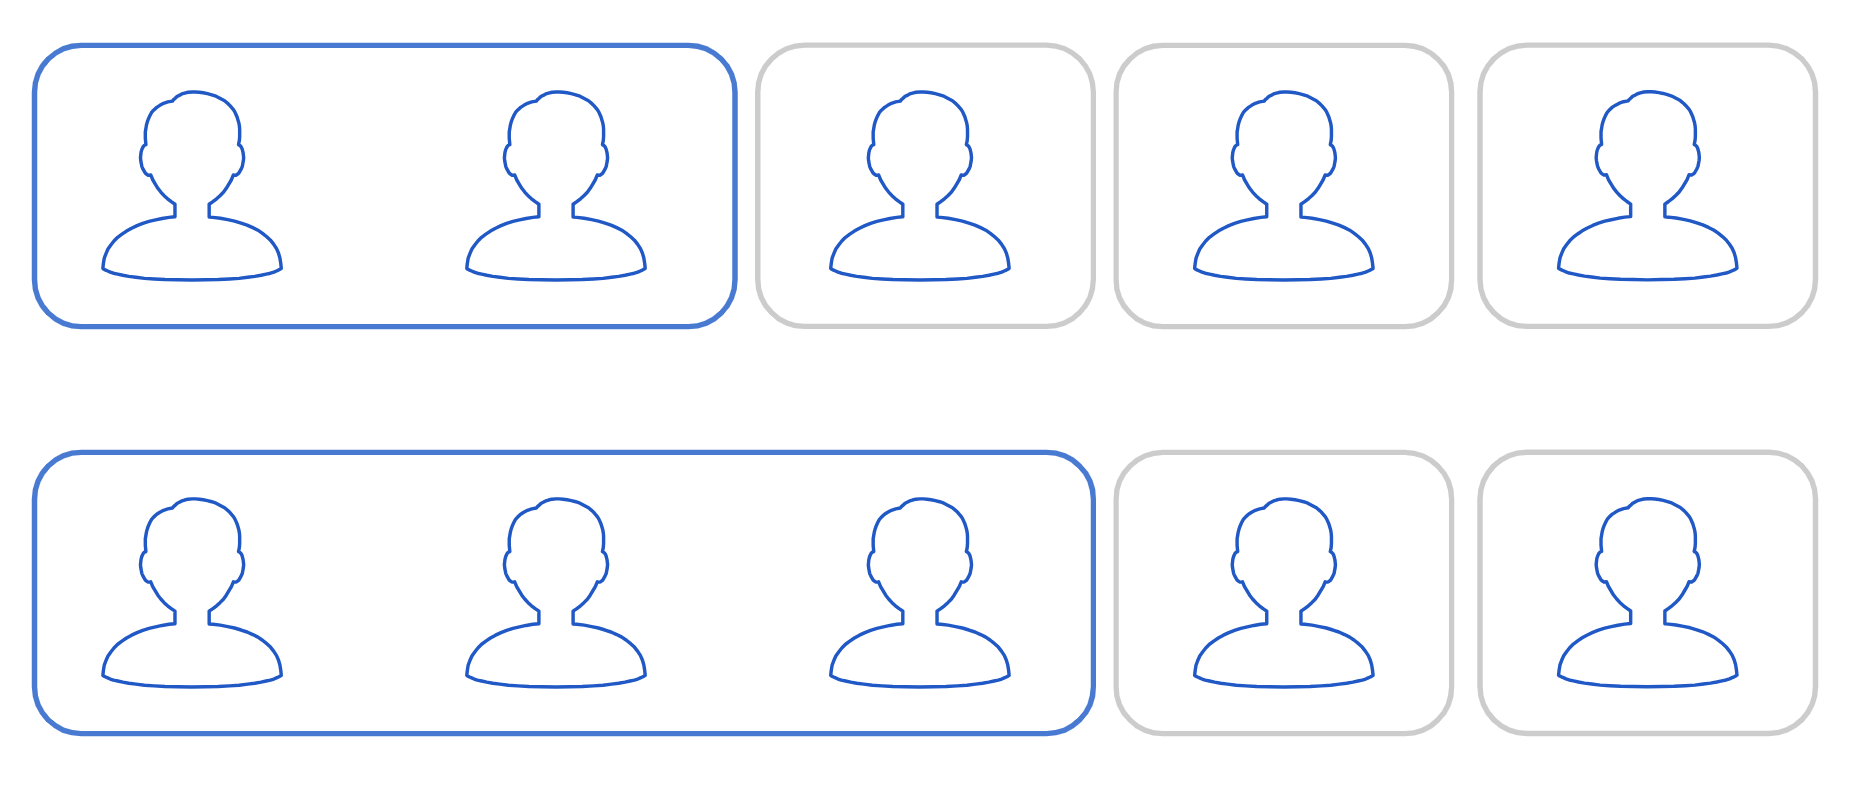
\includegraphics[scale = 0.4]{Static/dudes.png}
\end{center}

Illustrative example with 5 firms, where network expands from 2 firms to 3 firms 
    
\end{frame}


%\begin{comment}
    \begin{frame}{Estimation Results}

\begin{table}%[!htp]
%\caption{Estimation Results}\label{tab:estimation_results}
    \centering
    \begin{tabular}{lrc}
        \multicolumn{3}{c}{\textbf{Parameters}} \\
        Parameter & Value & Method \\
        \hline 
        Price Sensitivity $\alpha$ & -4 & Atalay et al (2023) \\ 
        Card Taste $\varsigma$ & 0.07 & Moments \\
        Cost Change $\zeta$ & -0.07 & Moments \\
        N Firms & 7 & Observed\\
        N Bank Networks & 1 & Observed\\ 
        Top Firm Share & 47\% & Observed\\
        Firm Store Card Share & 83\% & Observed\\
        Consumer Bank Card Share & 37\% & Observed \\
        \multicolumn{3}{c}{\textbf{Target Moments (My Estimates)}} \\
         Moment & Model & Data  \\
        \hline 
        $\Delta$ Store Card Share & -20\% & -20\% \\
        $\Delta$ Bank Card Share & +5.5\% & +5.5\% \\
        $\Delta SLS_{Notaccept}$  & +27bp & +27bp \\ 
        $\Delta SLS_{Accept}$ & -4.8\% & -4.8\% \\
    \end{tabular}
    %\caption{Caption}
\end{table} 

\end{frame}
%\end{comment}

\begin{frame}{Decomposing the Effect of Bank Cards}

\begin{table}[!htp]
    \centering
    \begin{tabular}{c|cccc}
    
        Variable &  Baseline & Treated & No Cost & Only Cost \\
        &&(Marquette) & Changes & Changes \\
        \hline 
        & (1) & (2) & (3) & (4)  \\
         Price Index &  1.24 & -66bp  & -21bp & -45bp \\
         Cost Index & 0.99 & -57bp  & 0 & -57bp \\
         Markup & 0.25 & -9bp & -21bp & +12bp \\
         %Producer Surplus & 0.23 & +4.2\% & -24bp & +4.5\% \\ 
         %Consumer Surplus & 0.75  & +2.9\% & -2.8bp & +2.9\% \\ 
         %Social Surplus & 0.98 & +3.2\% & -7.8bp & +3.3\% \\ 
    \end{tabular}
\end{table}
\end{frame}

%Stop being a pussy and just make this a bar graph 

\section{Implications for Regulators and Future Avenues for Research}
    \begin{frame}[noframenumbering, plain]
        \vfill
      \centering
      \begin{beamercolorbox}[sep=8pt,center,shadow=true,rounded=true]{title}
        \usebeamerfont{title}\insertsectionhead\par%
        \color{oxfordblue}\noindent\rule{10cm}{1pt} \\
      \end{beamercolorbox}
      \vfill
\end{frame}


\begin{frame}[label = regulation_uk]{UK Draft Legislation on BNPL}

UK draft legislation includes specific carve-out for merchant-funded credit: 

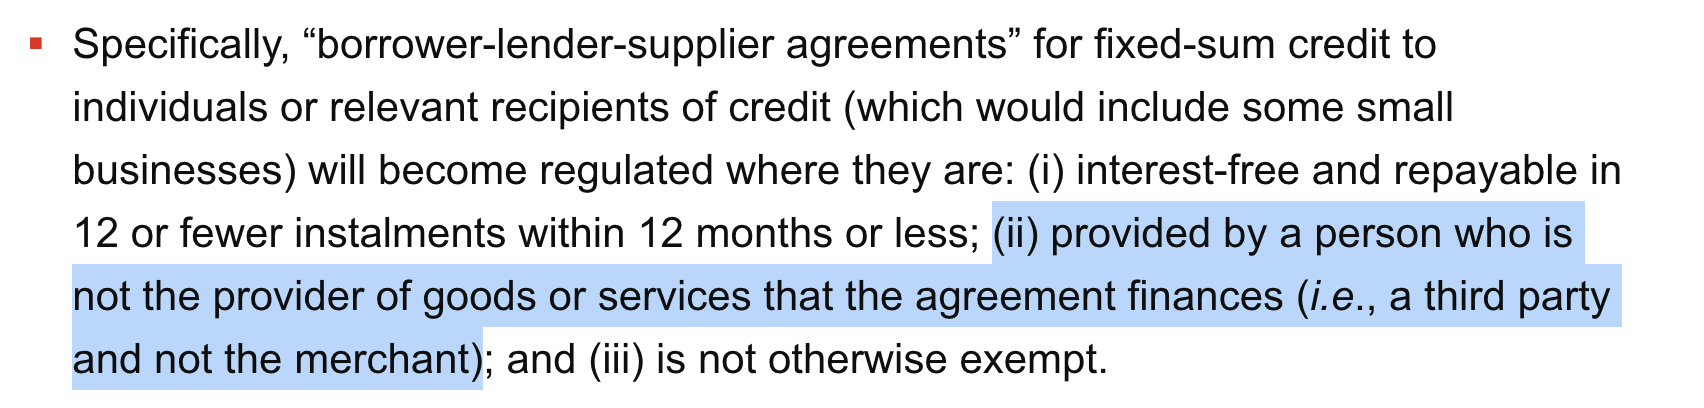
\includegraphics[scale = 0.5]{Static/regulation_uk.png}

(\cite{toms_uk})
\vfill 

Why force default risk to be held by retailers? 

%\hyperlink{literature}{\beamergotobutton{Back}}
    
\end{frame}

\begin{frame}{Developing Countries Still Rely on Store Lending}
    \begin{center}
    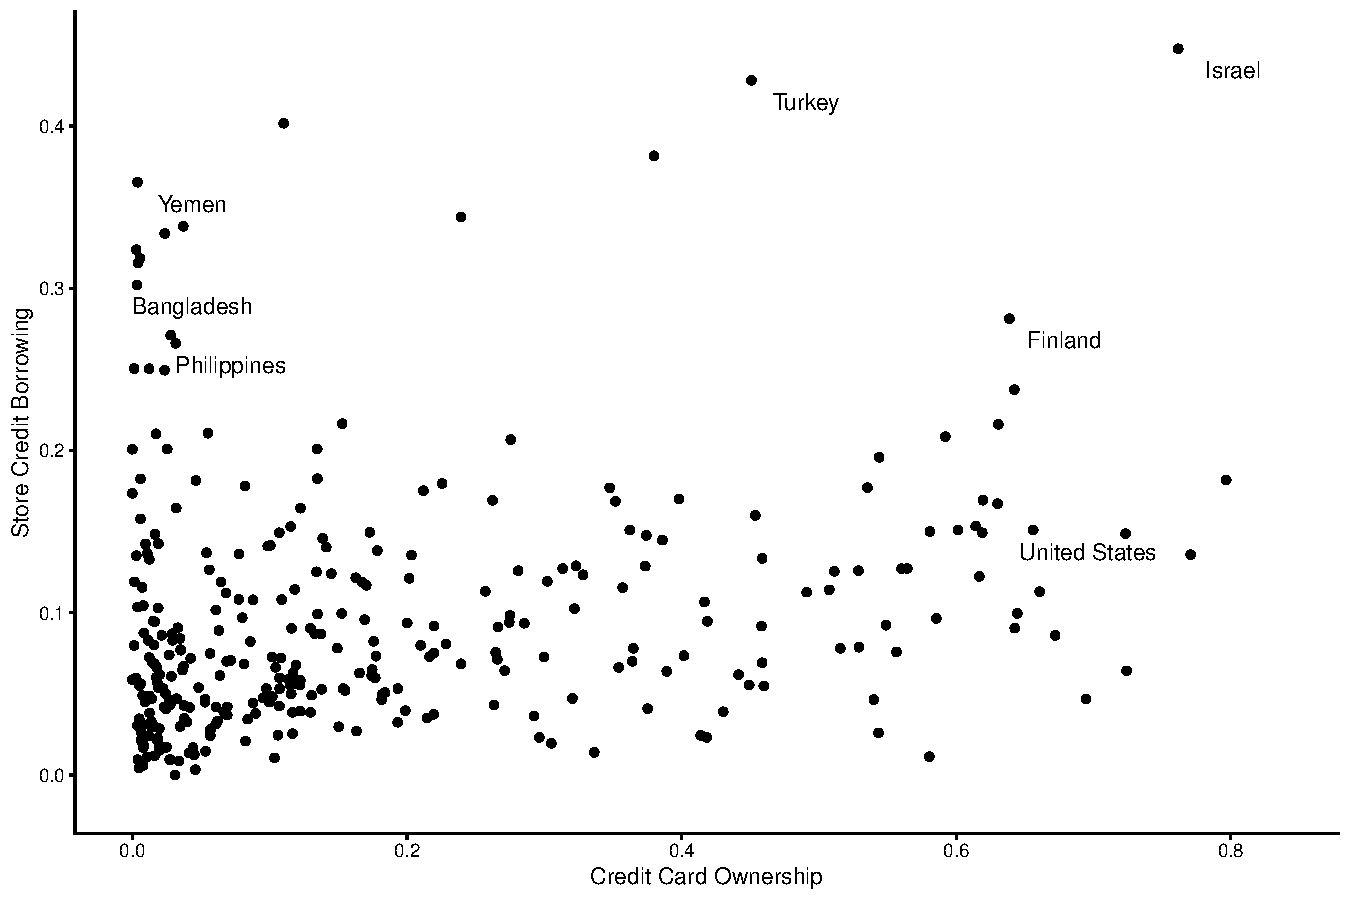
\includegraphics[scale = 0.45]{../Output/Figures/international.pdf}    
\end{center}
\vfill 
\resizebox{\dimexpr\paperwidth - 10ex}{!}{
Microcredit scholars attentive to store credit (\cite{field_repayment_2012}, \cite{cordaro_microequity_2022})
}
\end{frame}


\begin{frame}{Conclusion}

\begin{itemize}
    \item Nonfinancial retail merchants are a significant part of the consumer credit system and engage in ``regualatory arbitrage'' 
    \vfill 
    \item A monopolistic card network may still benefit merchants if it can better allocate real risk and real cost 
    \vfill 
    \item More research is needed on the outcomes of consumers who borrow from nonfinancial lenders, especially in developing countries  
\end{itemize}
\end{frame}


\begin{frame}{\centerline{Thank You!}}

\centering 

\includegraphics[scale = 0.4]{Static/thank_you.png}
    
\end{frame}

\begin{comment}
    \section{Thank You}
    \begin{frame}[noframenumbering, plain]
        \vfill
      \centering
      \begin{beamercolorbox}[sep=8pt,center,shadow=true,rounded=true]{title}
        \usebeamerfont{title}\insertsectionhead\par%
        \color{oxfordblue}\noindent\rule{10cm}{1pt} \\
      \end{beamercolorbox}
      \vfill
\end{frame}

\end{comment}




\begin{frame}[noframenumbering, label = coverage_time ]{USTD: Coverage Over Time}
\begin{centering}
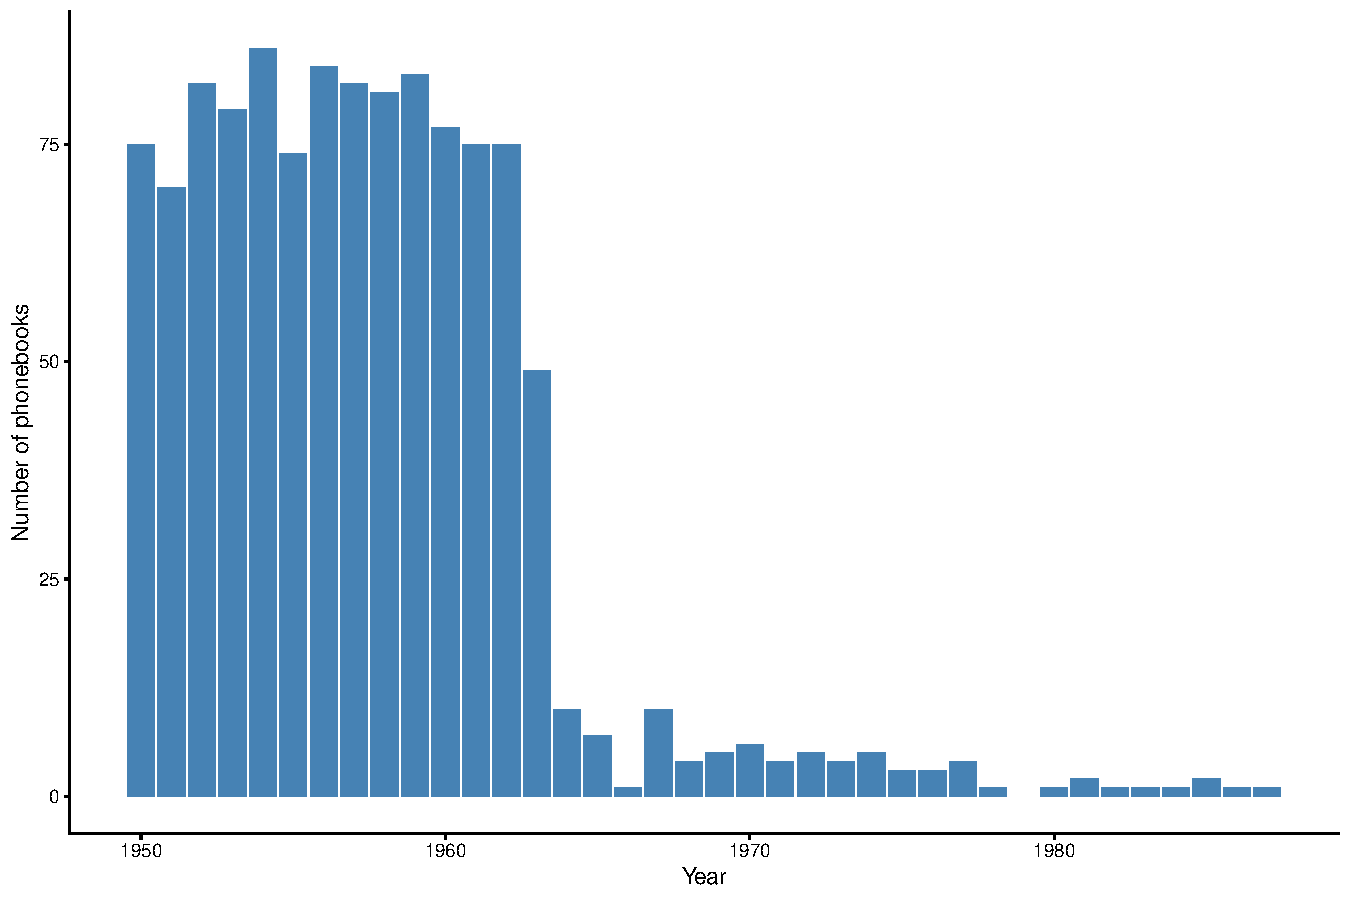
\includegraphics[scale = 0.4]{../Output/Figures/books_by_year.pdf} \\
\end{centering}

Number of Directories by Year in USTD Universe
\hyperlink{data_collection}{\beamergotobutton{Back}}
    
\end{frame}

\begin{frame}[noframenumbering, label = coverage_geographic]{USTD: Geographic Coverage}

\begin{centering}
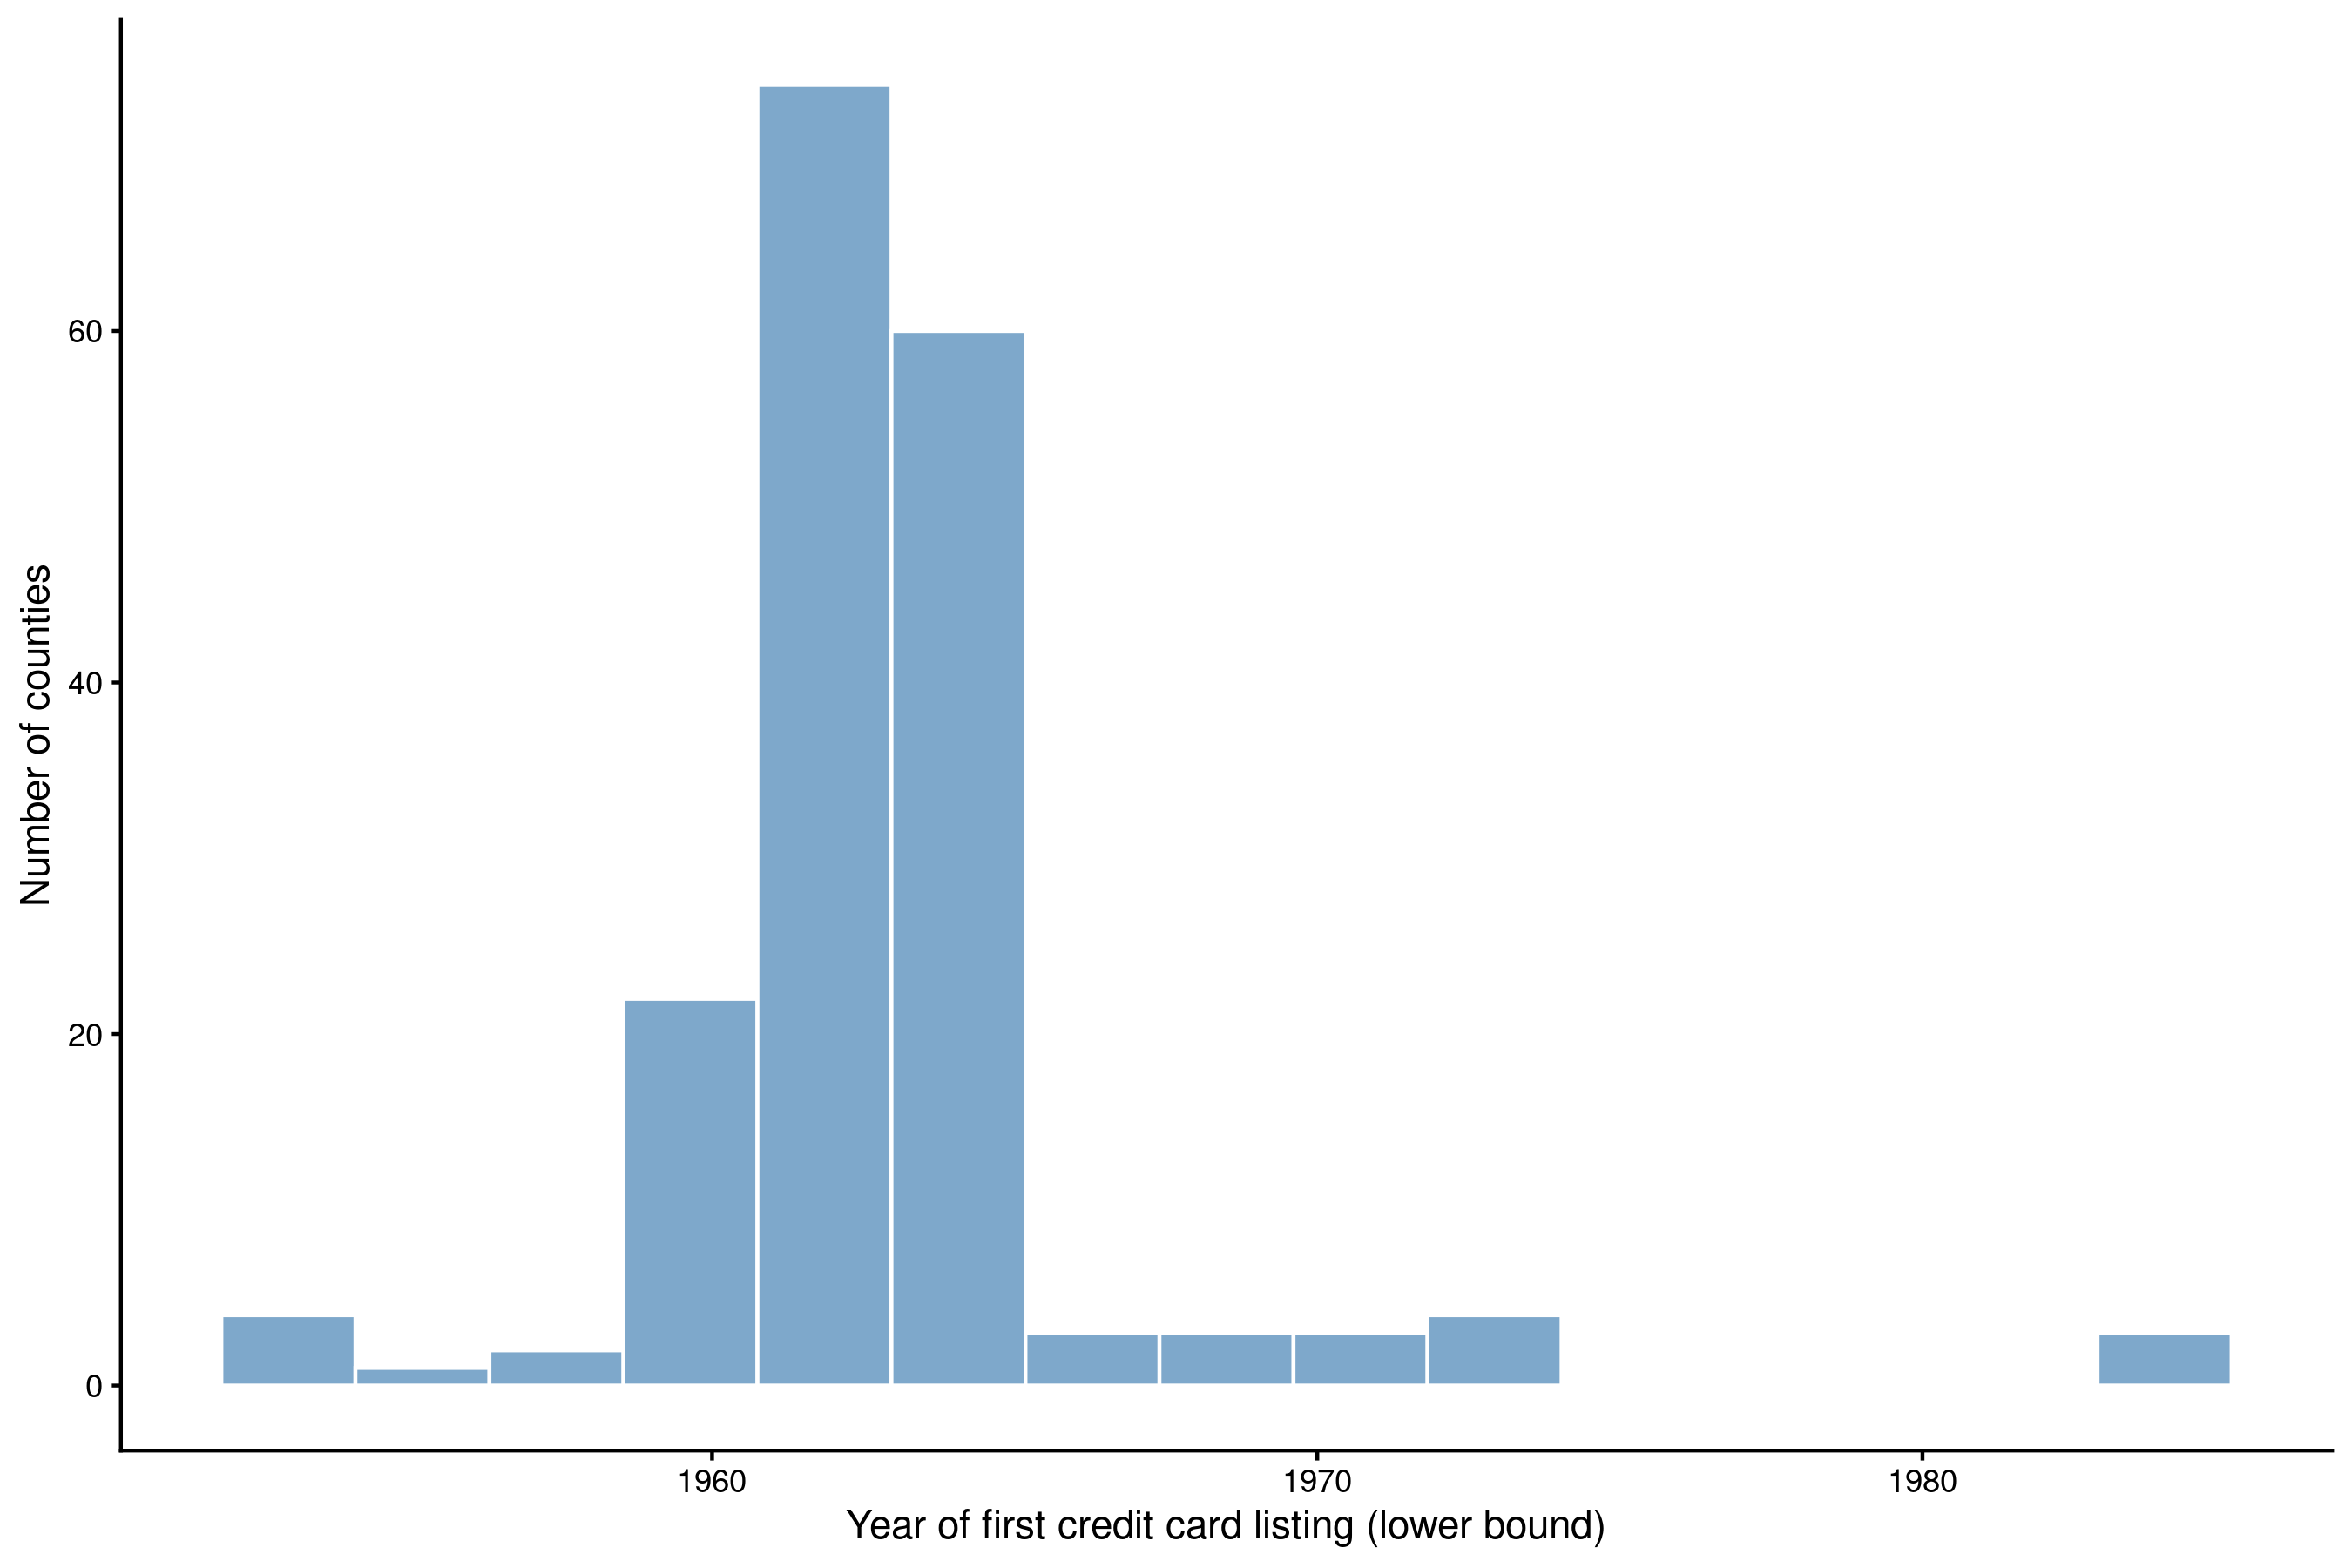
\includegraphics[scale = .4]{../Output/Figures/intro_lb.png} \\
\end{centering}    

Dates of Bank Card Introduction 
\hyperlink{data_collection}{\beamergotobutton{Back}}

\end{frame}


%\begin{frame}[allowframebreaks, noframenumbering]{References}
%        %\frametitle{References}
%        \bibliographystyle{authoryear}
%        \bibliography{references.bib}
%\end{frame}    


\end{document}